\chapter{Results}
\label{ch:results}

\section{Global Properties}
% To-Do:
% in general: more visual examples!
% Explicitly say the N_min and N_max
\subsection{Global Fractal Dimension}

To quantify the cloud morphology, we computed perimeter-area measurements over a restricted range of column densities, \(N_\mathrm{min} \leq N \leq N_\mathrm{max}\). This range was chosen to avoid biases caused by the limited angular resolution, which produces artificially smooth contours at low column densities, and by the sparse, irregular features that dominate at the highest column densities.

Figure~\ref{fig:orion_A_global} shows the perimeter-area relation for Orion~A, together with the best-fit linear regression in log-log space used to derive the global fractal dimension. The residuals of the fit are displayed in the lower panel. From this single-fit model we obtain:
\[
D_{\mathrm{OA,\,Global}} = 1.35 \pm 0.02 ,
\]
with a mean absolute residual of 0.1174 and a correlation coefficient of 0.9893.

\begin{figure}[t]
    \centering
    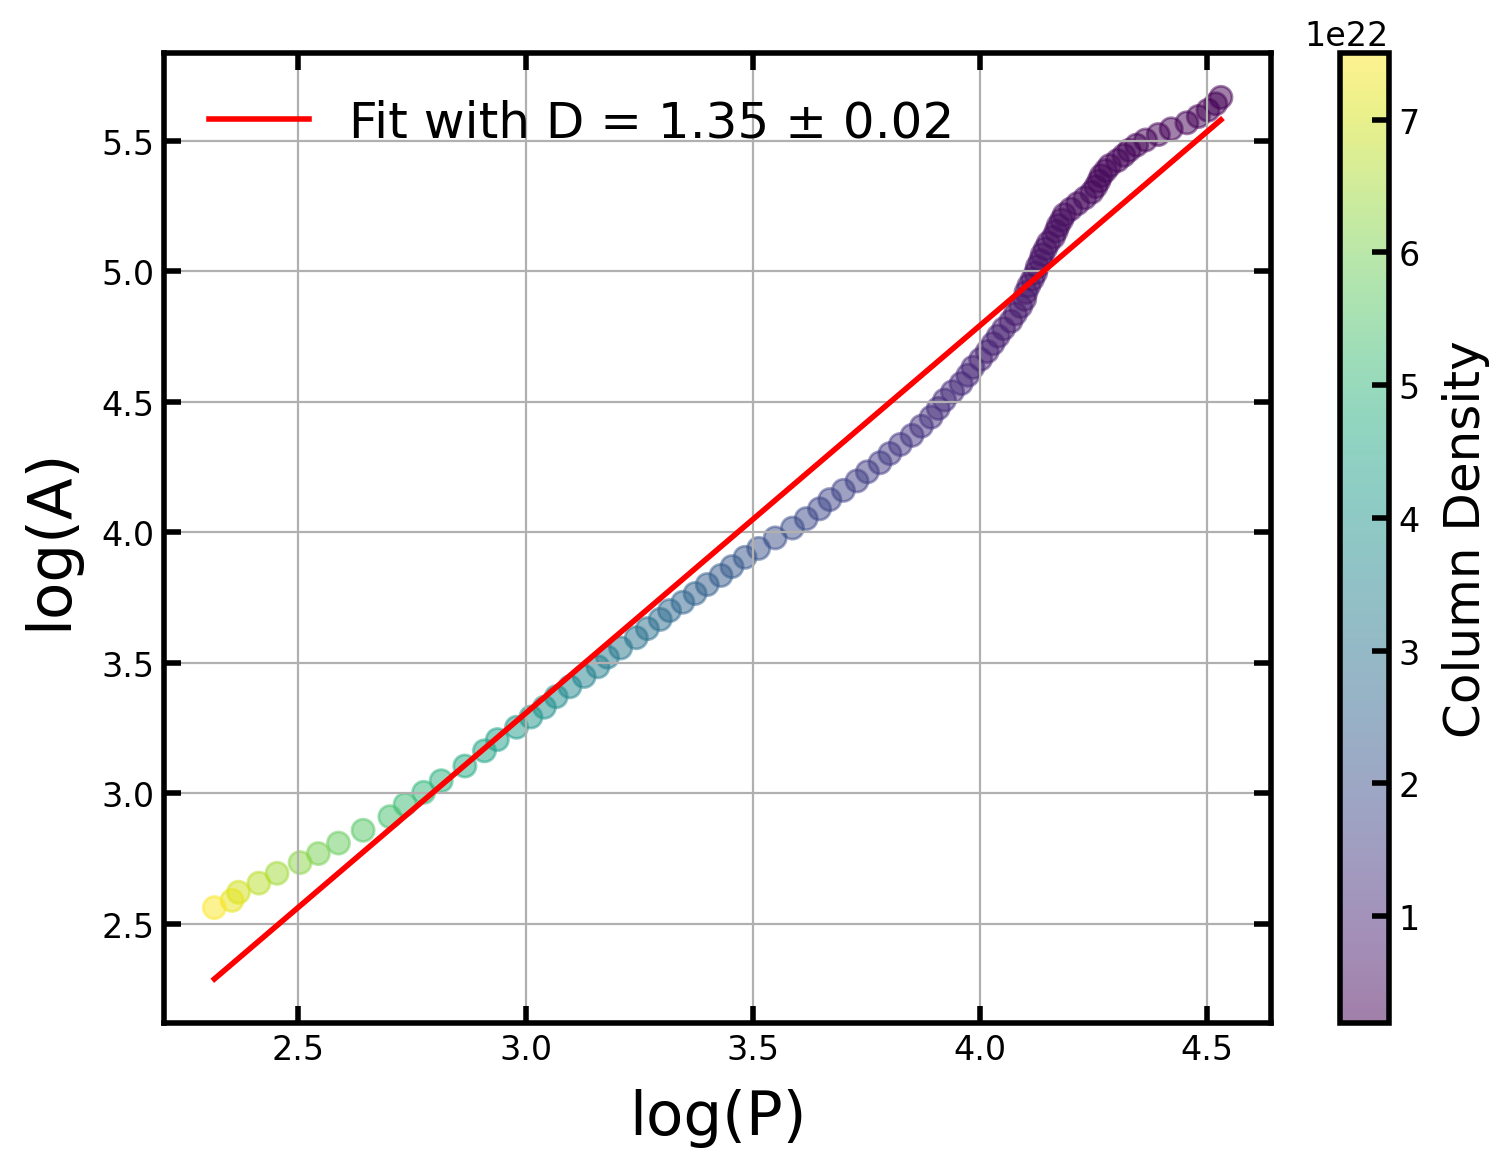
\includegraphics[width=0.5\textwidth]{figures/orion_A_global.png}
    \caption{Perimeter-area relation for Orion A. The solid line indicates the best-fit linear regression in log--log space used to estimate the global fractal dimension \(D\). Residuals are shown in the lower panel.}
    \label{fig:orion_A_global}
\end{figure}

However, the Orion A data show systematic deviations from a single power law across the full column-density range. To account for this, we performed a segmented (double) linear fit, dividing the data at \(N = 1.23 \times 10^{22}\,\mathrm{cm}^{-2}\). The two resulting slopes are:
\[
D_1 = 1.65 \pm 0.01 \quad \text{(high column density)},
\]
\[
D_2 = 0.97 \pm 0.02 \quad \text{(low column density)}.
\]
The corresponding mean absolute residuals are 0.0222 (correlation coefficient = 0.9986) for the high-density regime and 0.0679 (correlation coefficient = 0.9748) for the low-density regime, representing a clear improvement compared to the single-fit model.  
Figure~\ref{fig:orion_A_global_double_fit} shows the two fitted segments and their residuals. The distinct change in slope suggests a structural transition or the coexistence of different regimes of spatial complexity in Orion~A.

\begin{figure}[t]
    \centering
    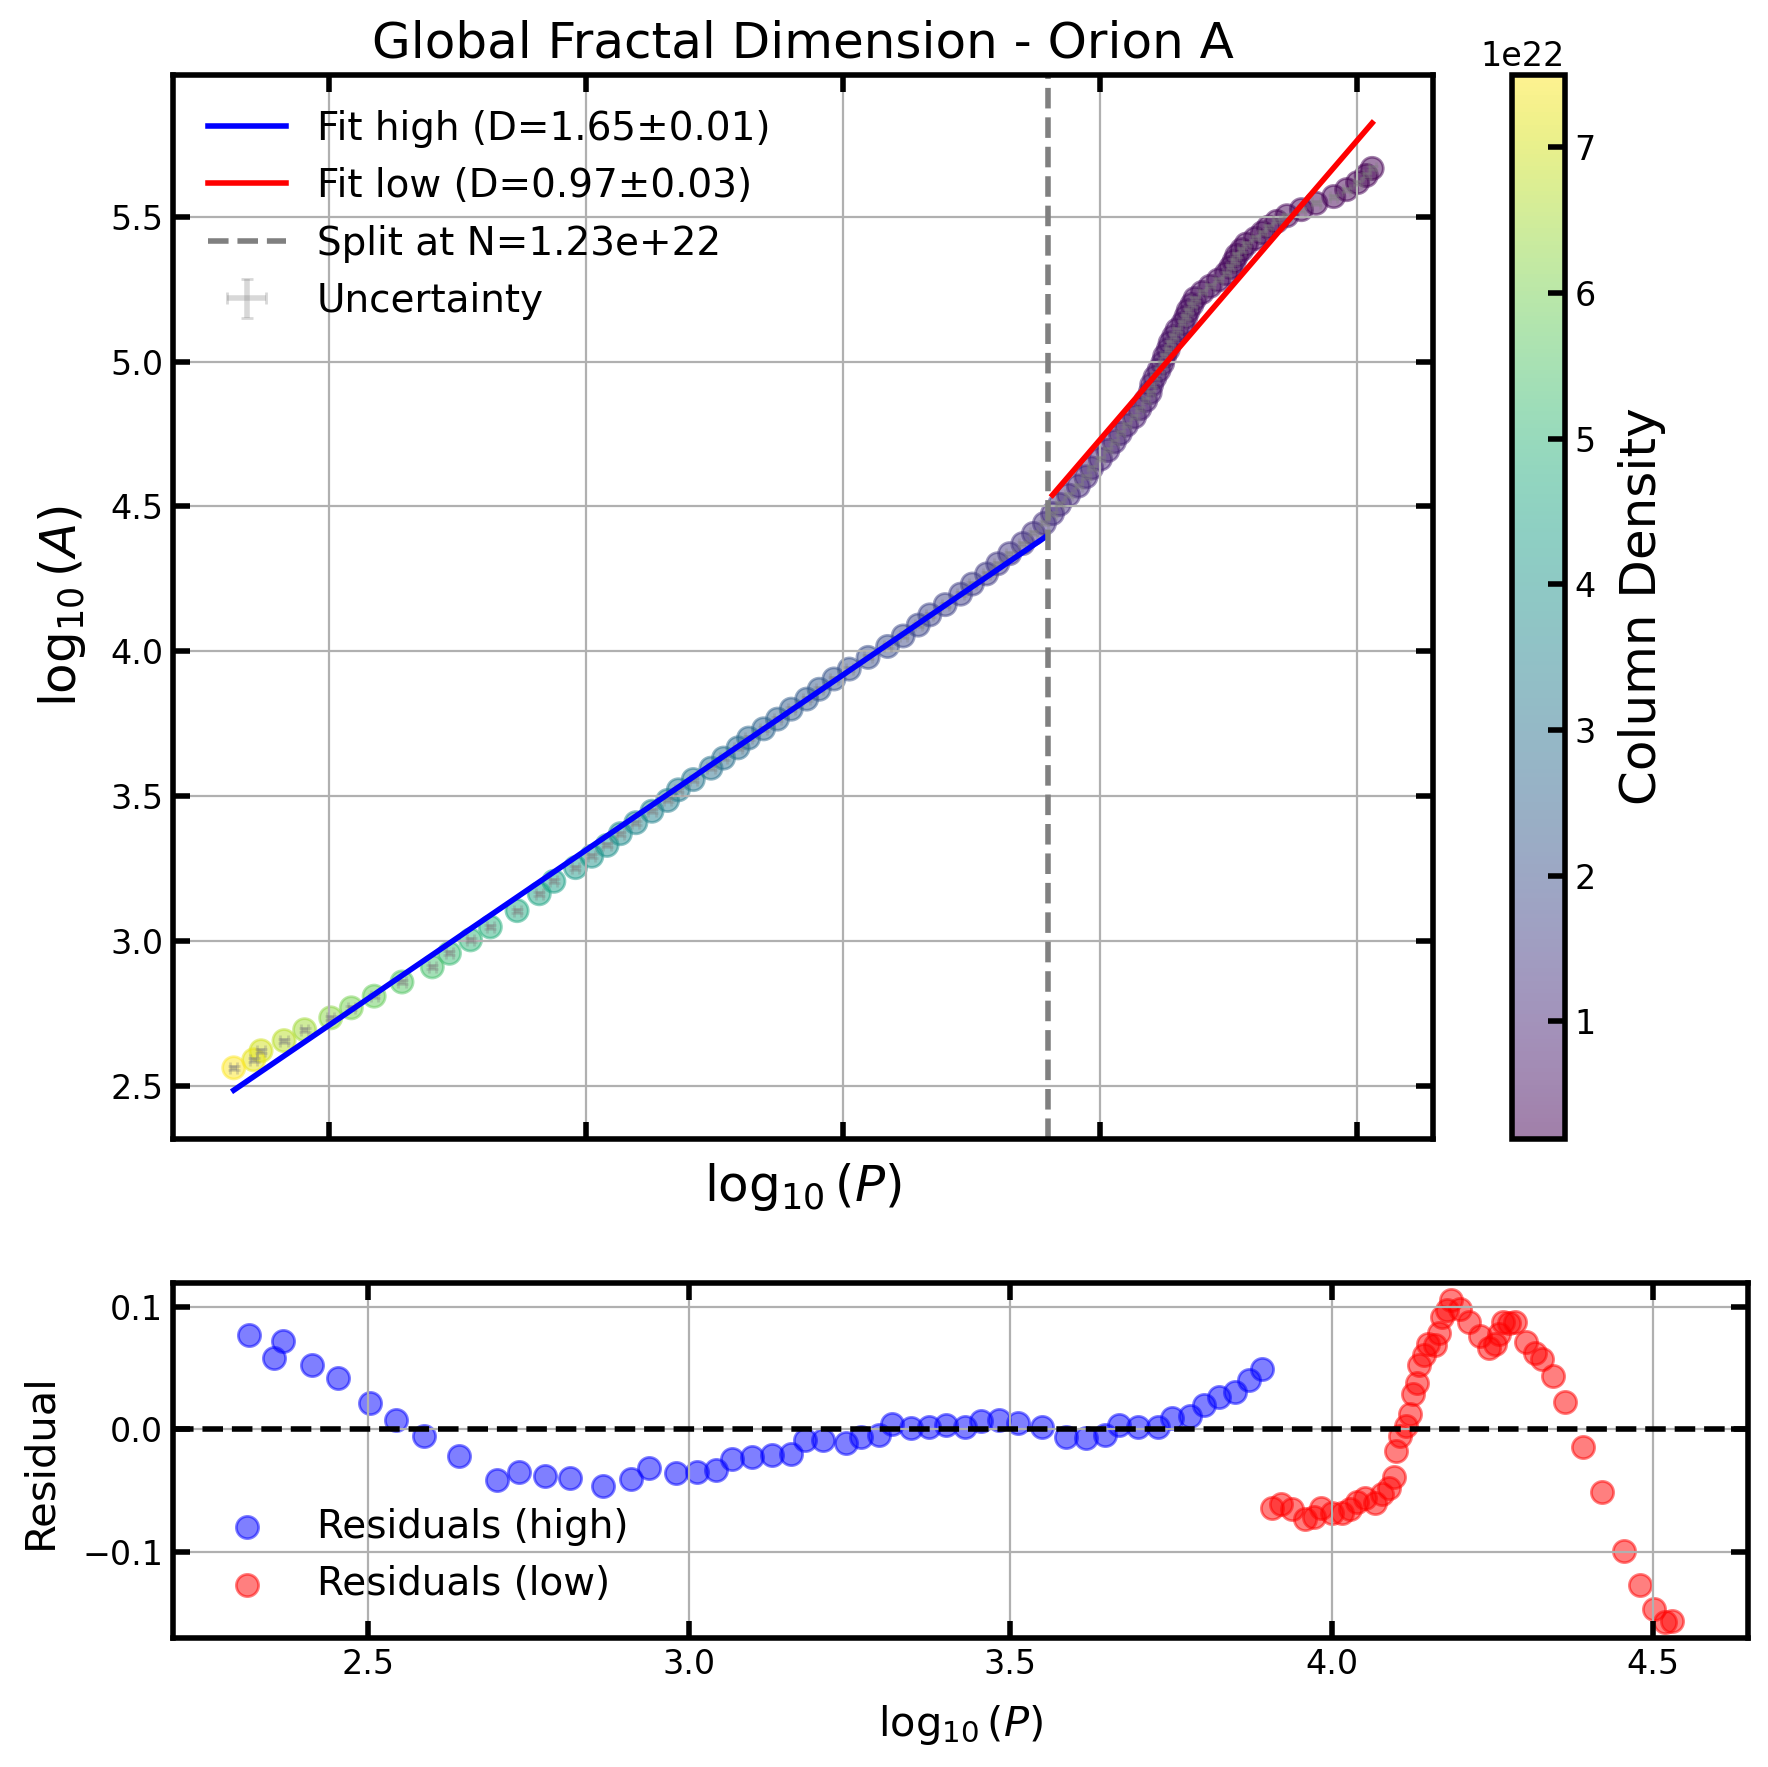
\includegraphics[width=0.5\textwidth]{figures/orion_A_global_double_fit.png}
    \caption{Perimeter-area relation for Orion~A with a segmented linear fit. Dashed lines indicate the two fitted regimes, separated at \(N = 1.23 \times 10^{22}\,\mathrm{cm}^{-2}\). Residuals are shown in the lower panel.}
    \label{fig:orion_A_global_double_fit}
\end{figure}

In contrast, Orion~B exhibits a well-behaved perimeter-area relation that is accurately described by a single linear fit across the entire column-density range:
\[
D_{\mathrm{OB,\,Global}} = 1.40 \pm 0.01 .
\]
The corresponding residuals (mean absolute residual = 0.0493) and correlation coefficient (0.9976) confirm the robustness of this fit. Figure~\ref{fig:orion_B_global} shows the fitted relation and residuals. The consistency of the slope across scales indicates a more uniform degree of structural complexity compared to Orion~A.

\begin{figure}[t]
    \centering
    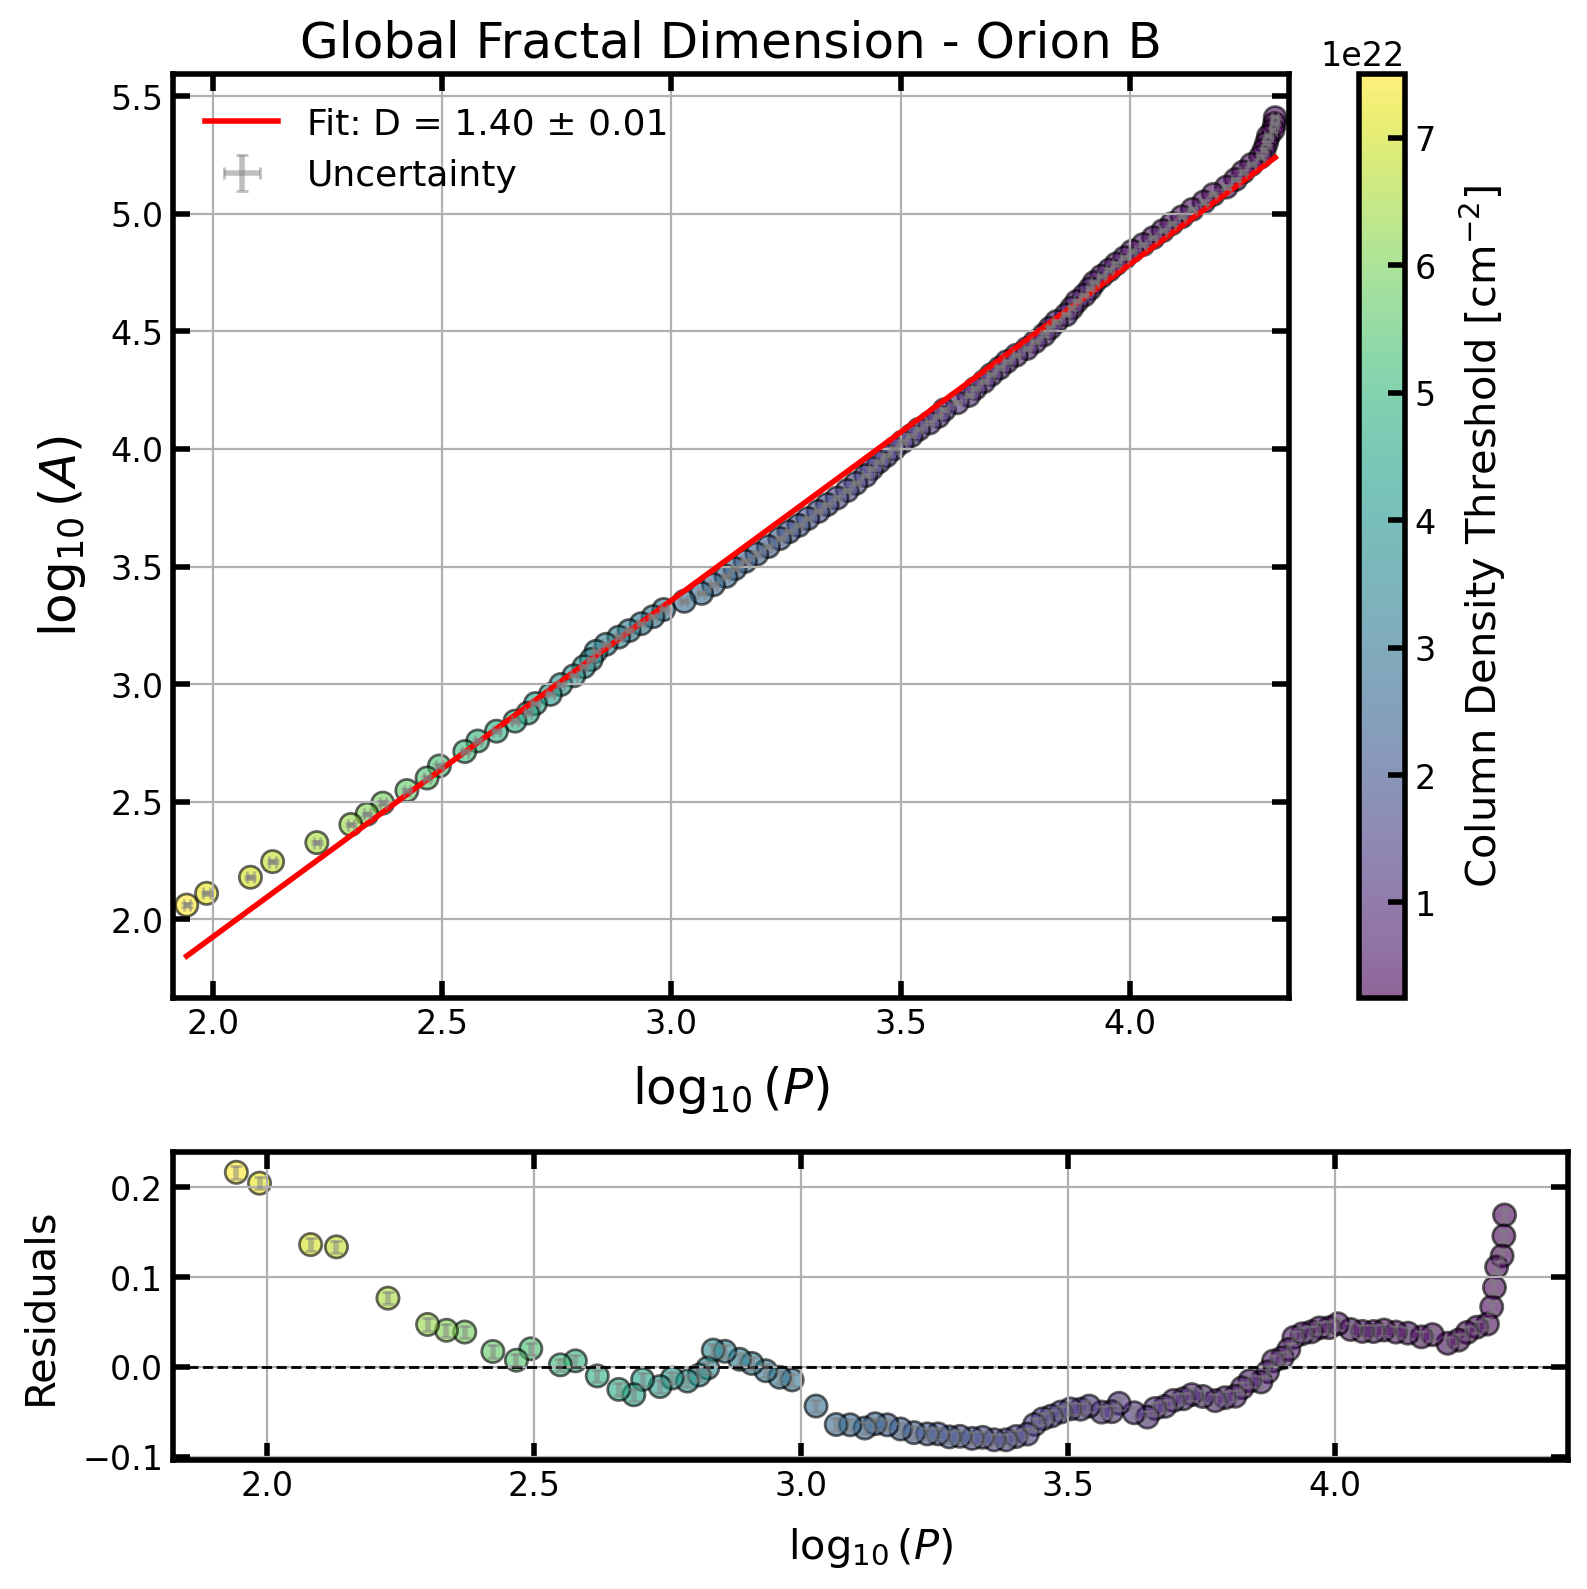
\includegraphics[width=0.5\textwidth]{figures/orion_B_global.png}
    \caption{Perimeter-area relation for Orion~B with the best-fit linear regression overlaid. Residuals are shown in the lower panel.}
    \label{fig:orion_B_global}
\end{figure}

The uncertainties in perimeter and area measurements were estimated at 1.6\%, based on simulations demonstrating that this level of error is representative across different reference geometries.

% To-Do:
% Explicitly say the N_min and N_max
\section{Local Properties}

\subsection{Euler Characteristic}

We evaluated the Euler characteristic, \(\chi\), for both Orion~A and Orion B as a function of the column–density threshold. This topological descriptor quantifies the connectivity and fragmentation of structures within the clouds: larger positive values of \(\chi\) indicate a predominance of isolated regions, while more negative values reflect a higher degree of connectivity.

Figures~\ref{fig:Euler_Orion_A_no_figs} and~\ref{fig:Euler_Orion_B_no_figs} present the results for Orion A and Orion B, respectively. In each case, \(\chi\) was computed over the same range of column densities used in the perimeter–area analysis, ensuring consistency.

\begin{figure}[t]
    \centering
    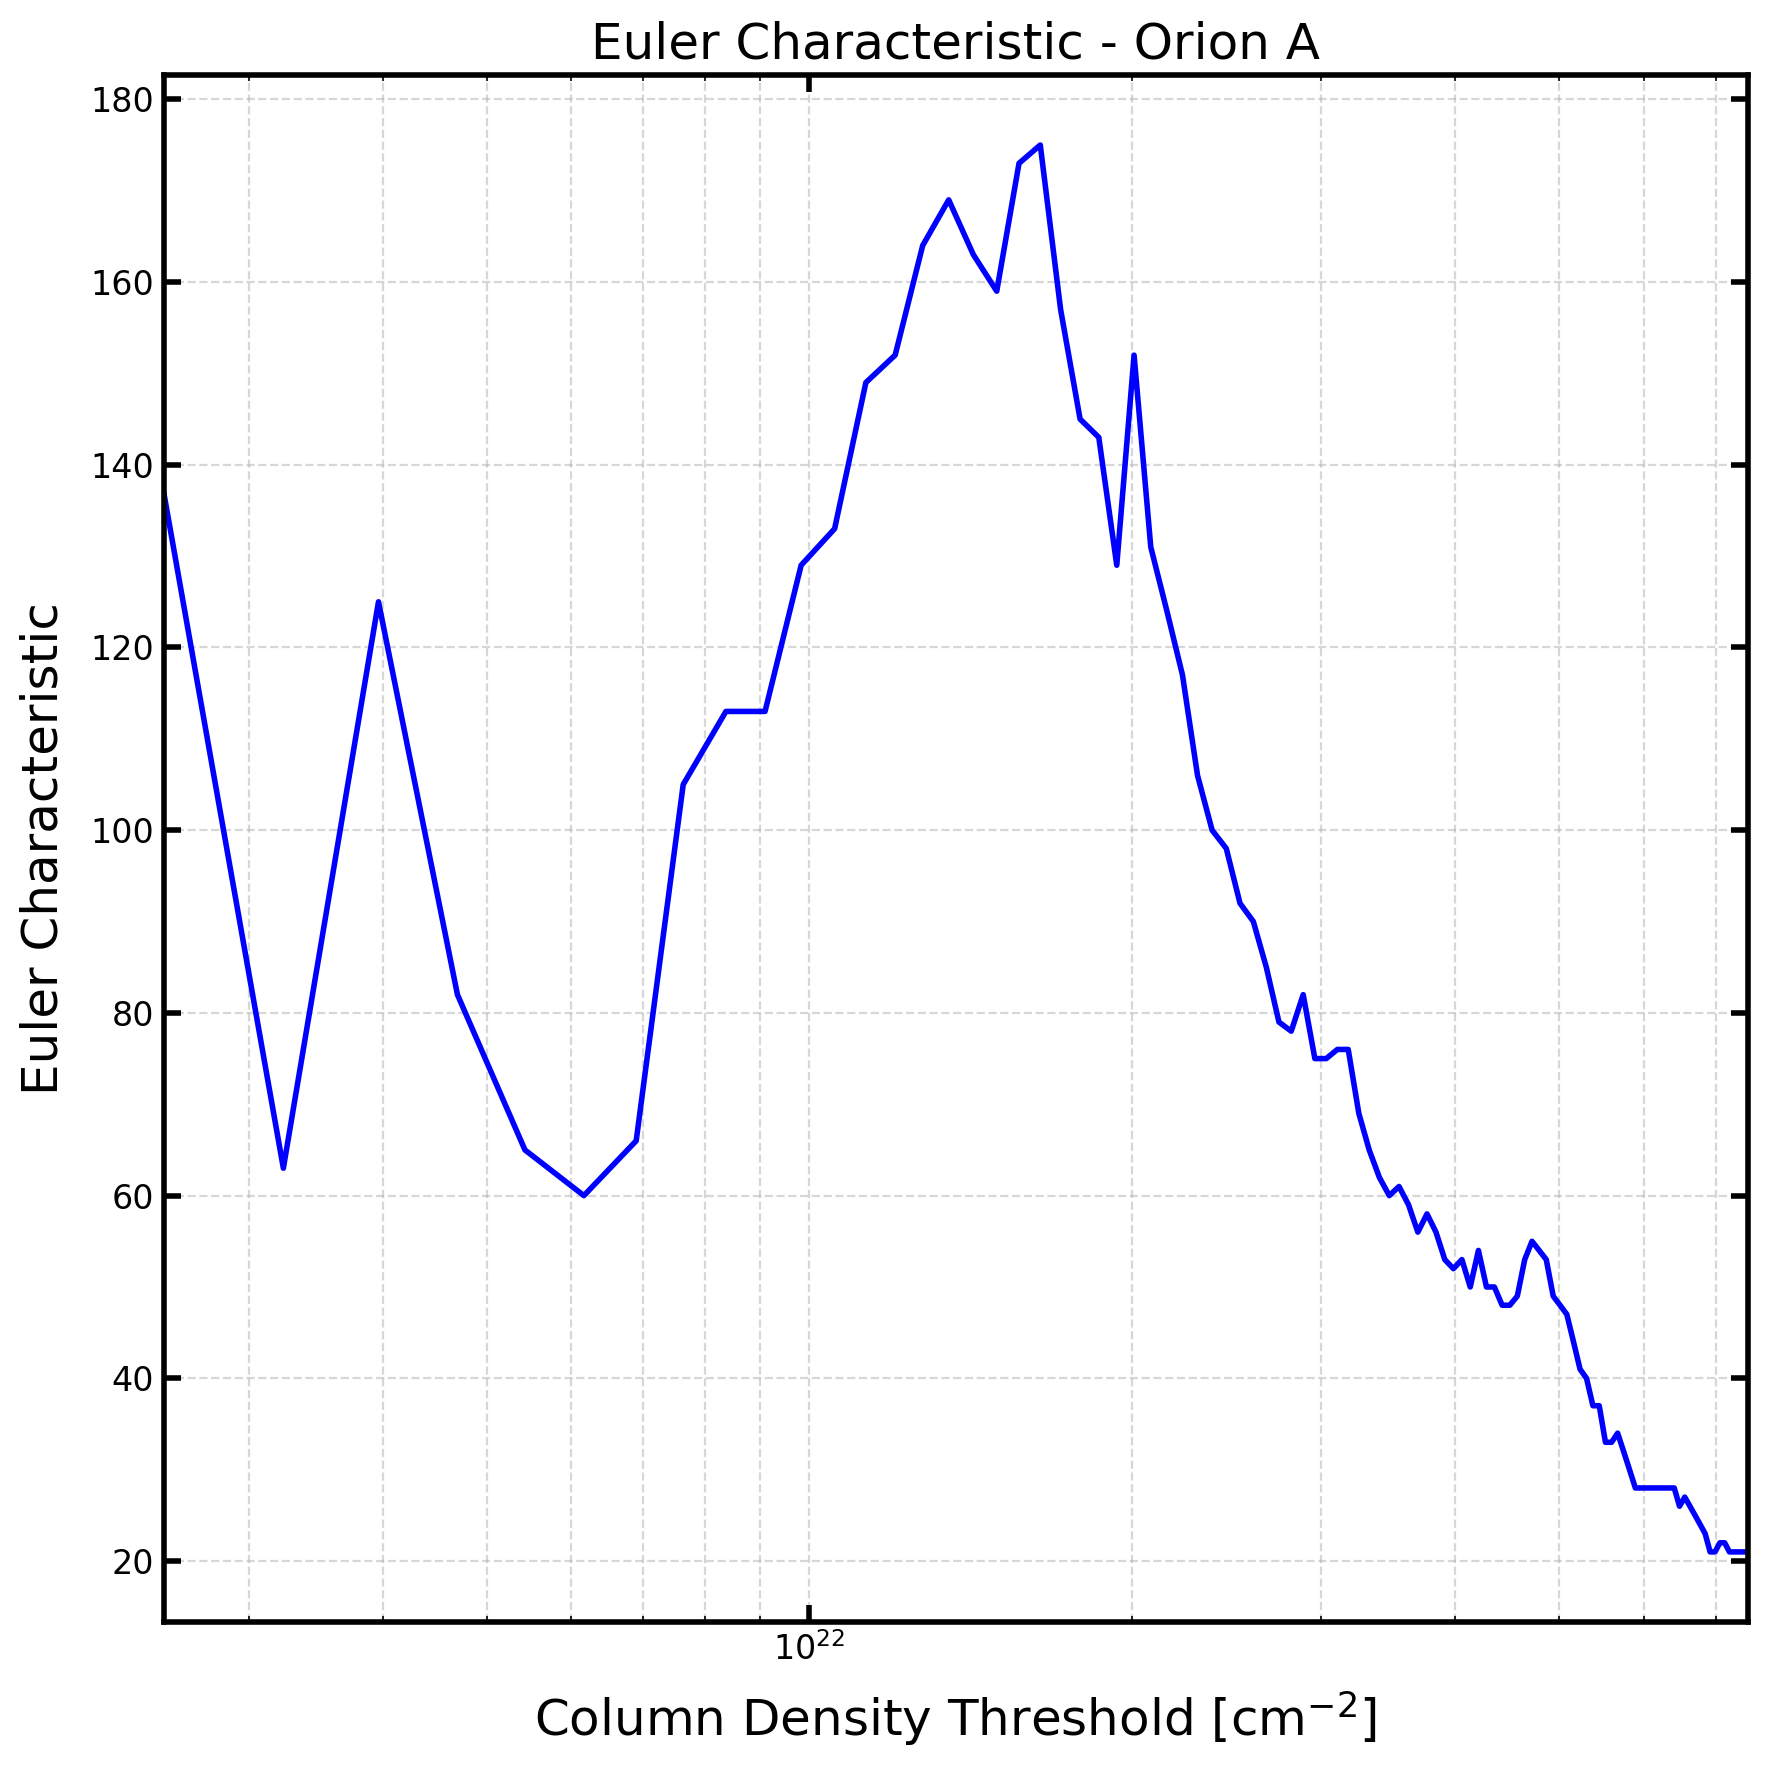
\includegraphics[width=0.5\textwidth]{figures/euler_Orion_A_no_figs.png}
    \caption{Euler characteristic of Orion~A as a function of column–density threshold. Positive values correspond to a predominance of isolated structures, while negative values indicate higher connectivity.}
    \label{fig:Euler_Orion_A_no_figs}
\end{figure}

\begin{figure}[t]
    \centering
    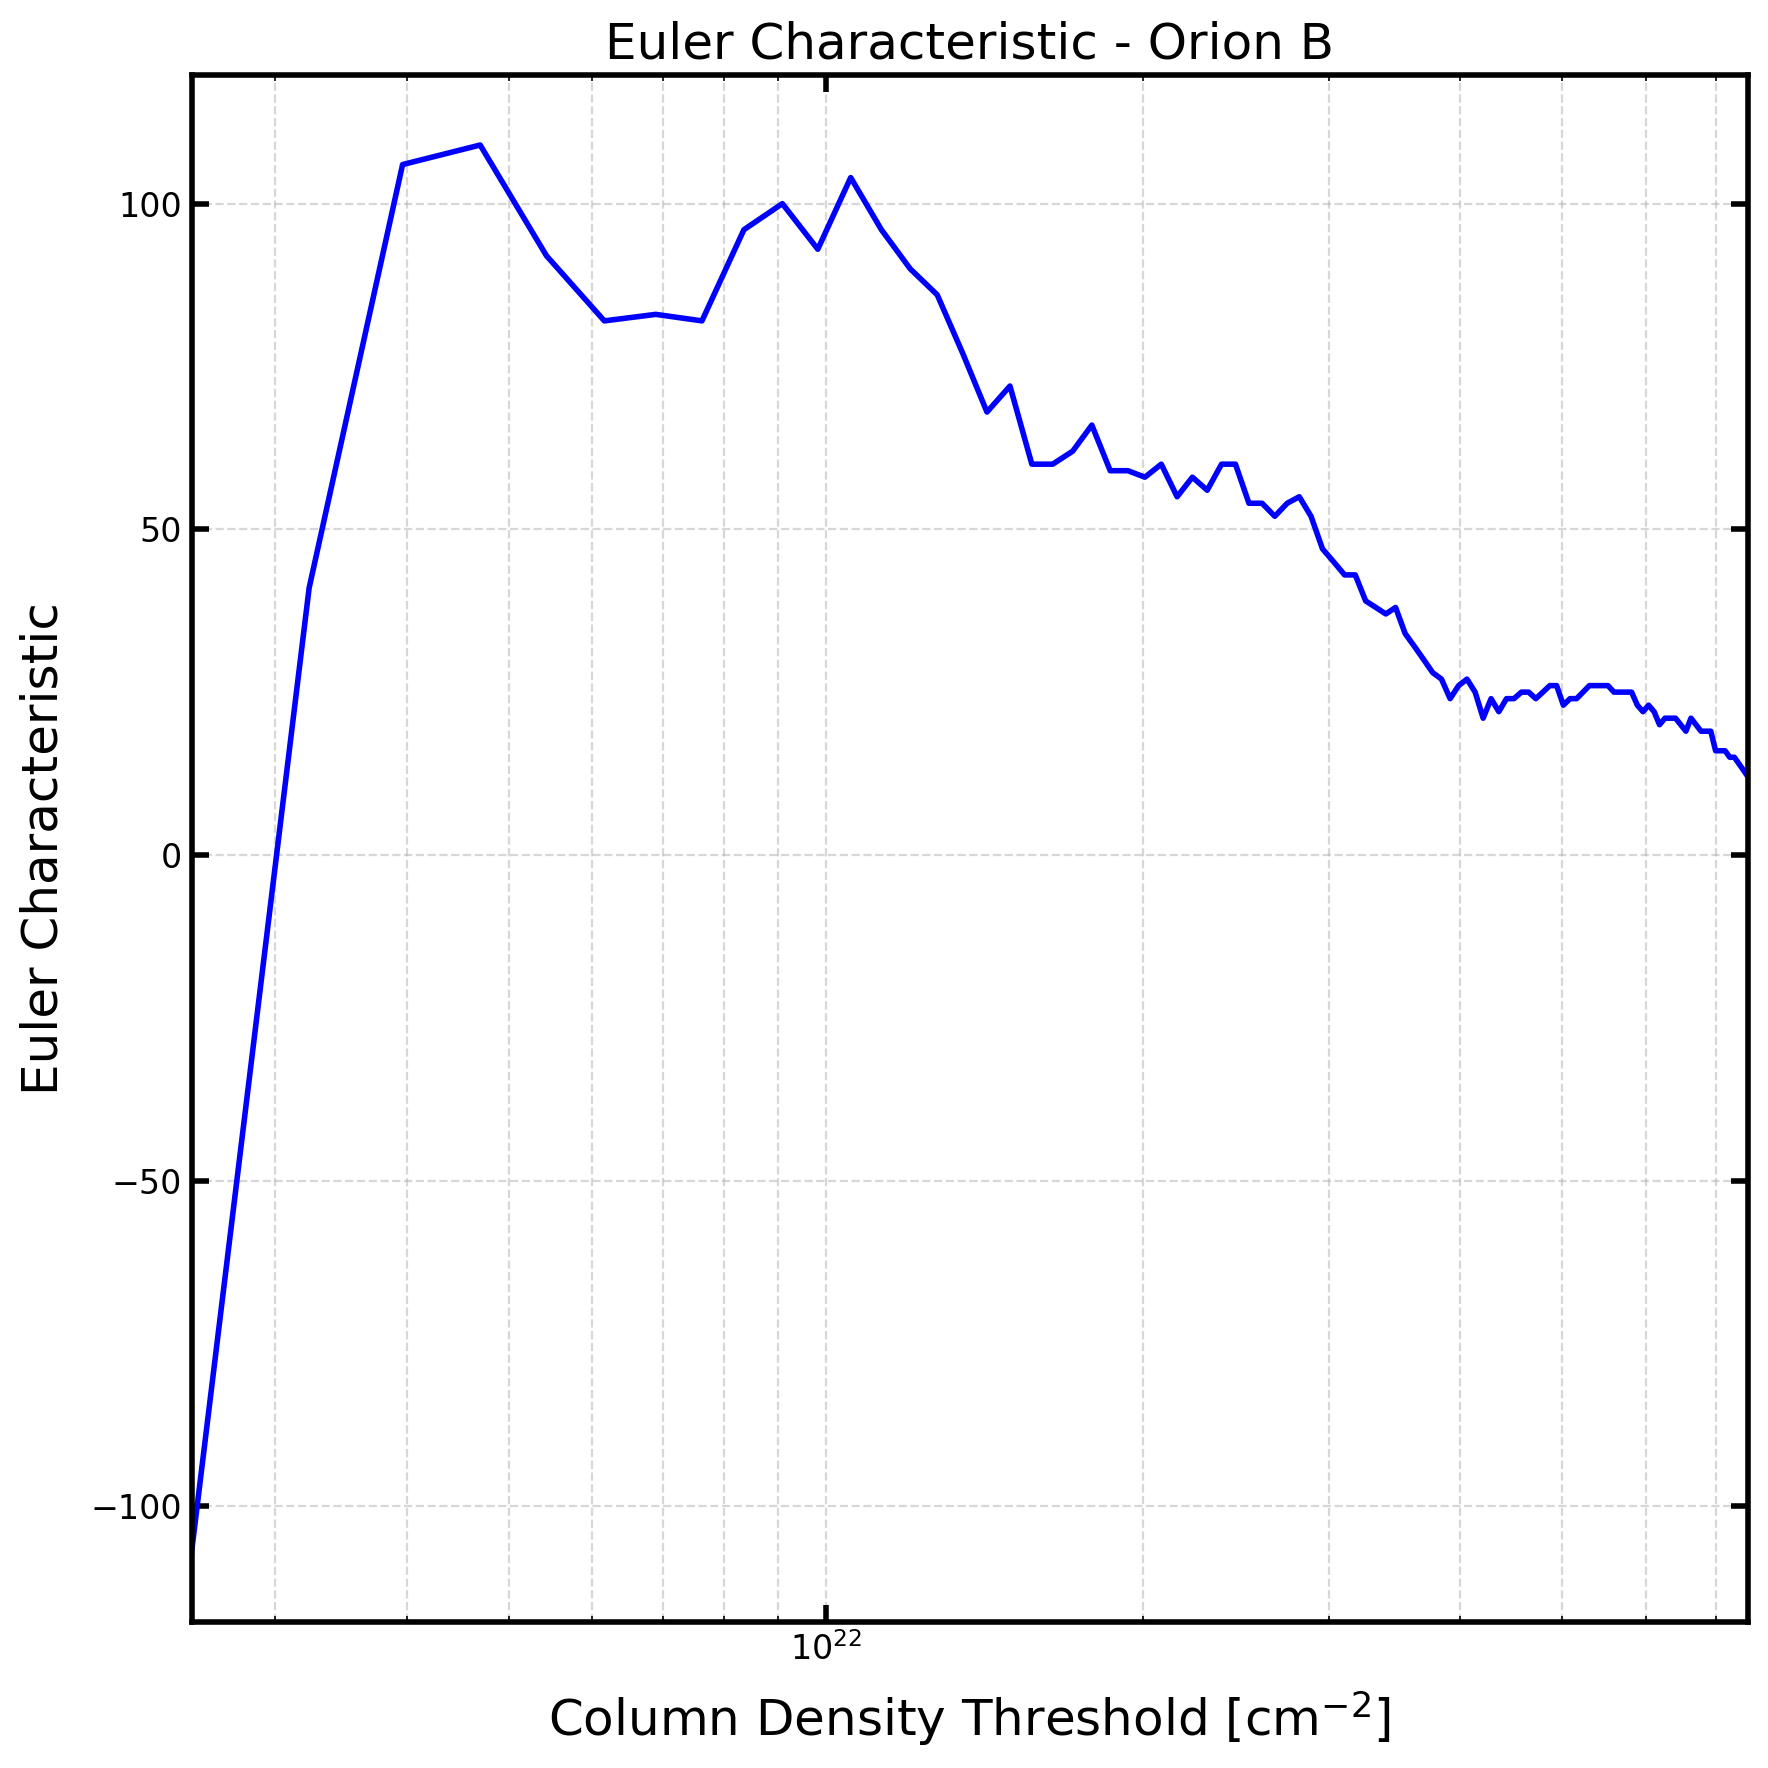
\includegraphics[width=0.5\textwidth]{figures/euler_Orion_B_no_figs.png}
    \caption{Euler characteristic of Orion~B as a function of column–density threshold.}
    \label{fig:Euler_Orion_B_no_figs}
\end{figure}

\subsection{Local Fractal Dimension}

Figure~\ref{fig:local_Orion_A_B} shows the variation of the local fractal dimension as a function of column--density threshold for Orion~A and Orion~B. In both regions we find a clear overall trend: the local fractal dimension changes systematically as the threshold increases. Superimposed on this trend, several pronounced peaks and deviations are visible. These features likely trace transitions in the morphology of the structures, for instance the emergence of compact cores or the fragmentation of filaments into smaller substructures.

A more detailed interpretation of these peaks and their implications for cloud evolution and turbulence will be addressed in the following sections. In particular, we will assess whether these variations represent genuine structural changes or arise from limitations such as resolution effects and increased noise at higher thresholds.

\begin{figure}[t]
    \centering
    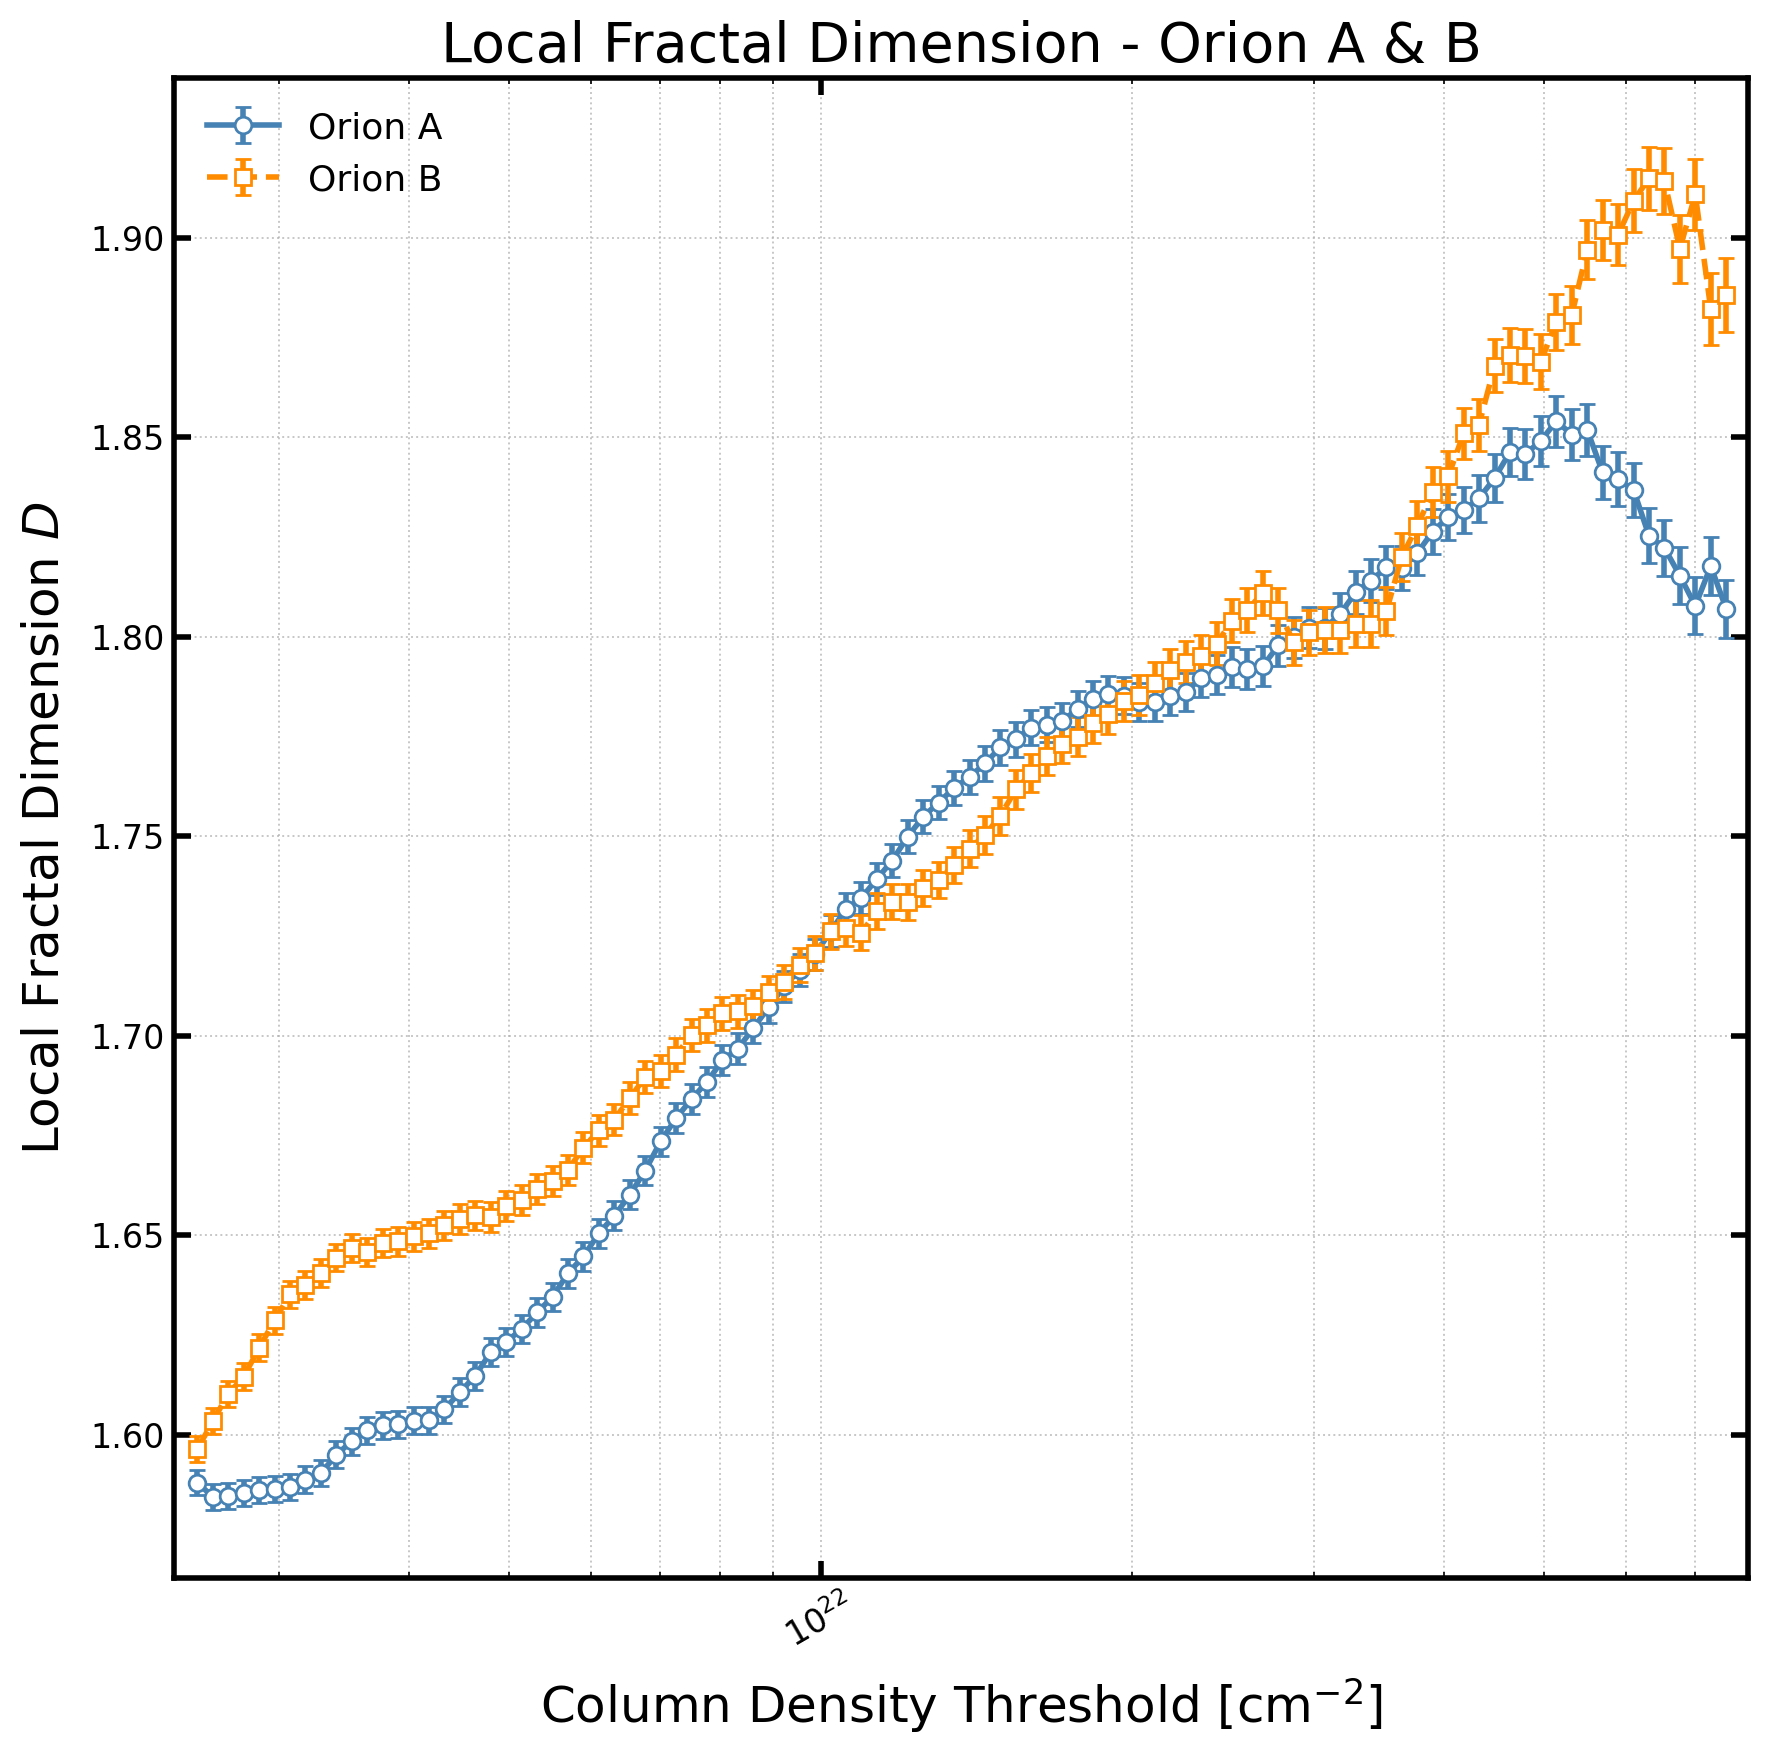
\includegraphics[width=0.5\textwidth]{figures/local_orion_A_B.png}
    \caption{Local fractal dimension as a function of column--density threshold for Orion~A and Orion~B. Error bars reflect the uncertainties of the fit at each threshold.}
    \label{fig:local_Orion_A_B}
\end{figure}

\subsection{Analysis of Individual Structures}

To gain deeper insight into the fractal properties of each cloud, we decomposed the emission at every column--density threshold into its set of connected structures. This dendrogram--based approach provides a hierarchical view of how the material is organized into nested substructures, enabling a more detailed examination of their geometrical and topological properties.

Figures~\ref{fig:dendrogram_A} and~\ref{fig:dendrogram_B} display the resulting dendrograms for Orion~A and Orion~B. These diagrams trace how individual regions merge into larger complexes as the threshold decreases, effectively capturing the clustering behaviour of the cloud across spatial scales.

\begin{figure}[t]
    \centering
    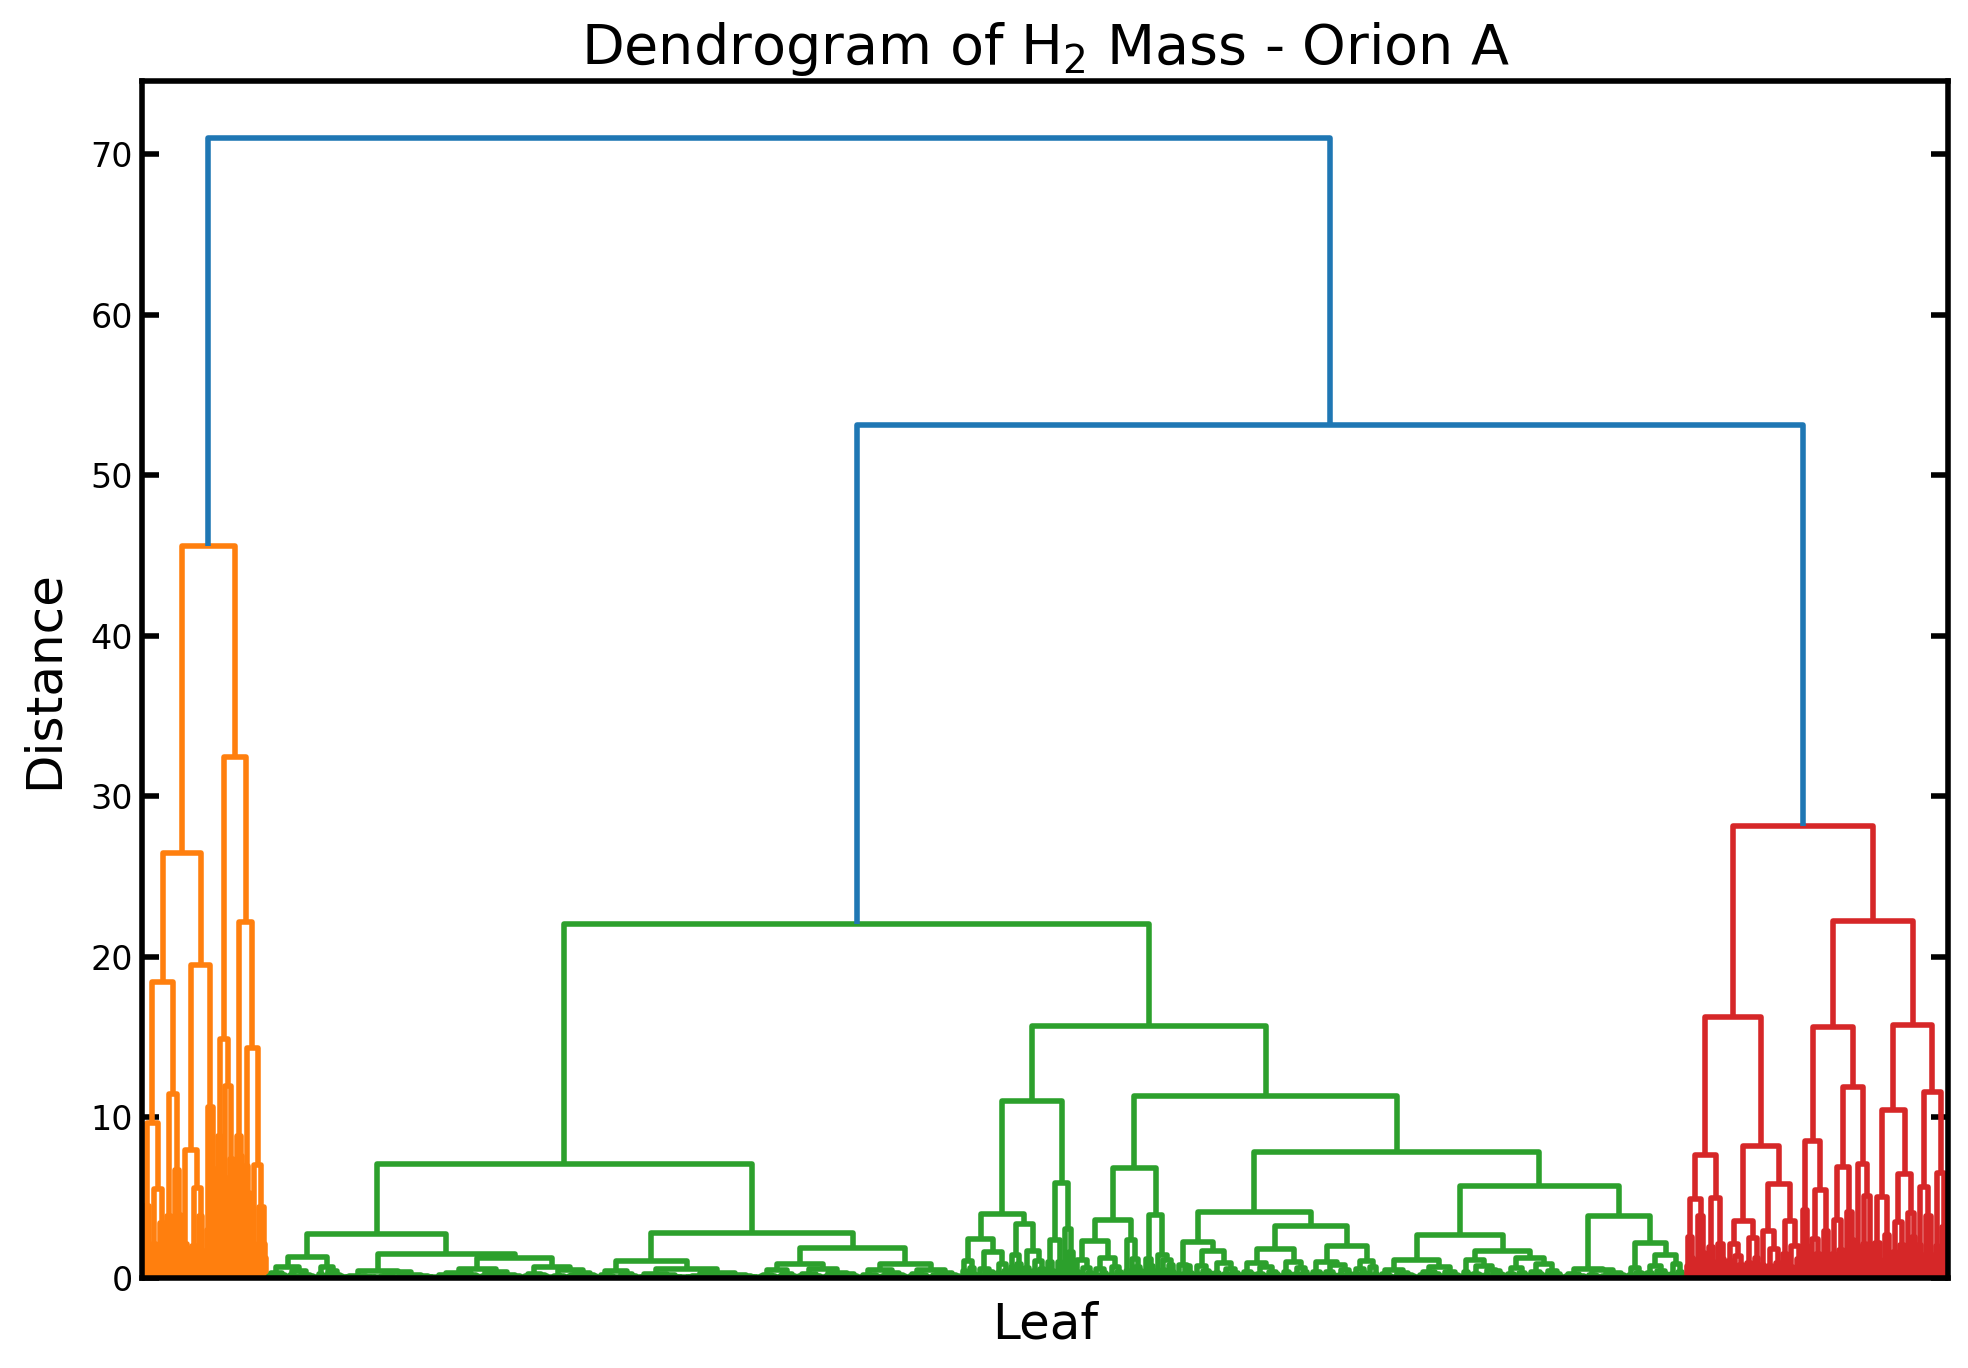
\includegraphics[width=0.5\textwidth]{figures/dendogram_A.png}
    \caption{Dendrogram of the Orion~A mass distribution, showing the hierarchical merging of structures as the column--density threshold is lowered.}
    \label{fig:dendrogram_A}
\end{figure}

\begin{figure}[t]
    \centering
    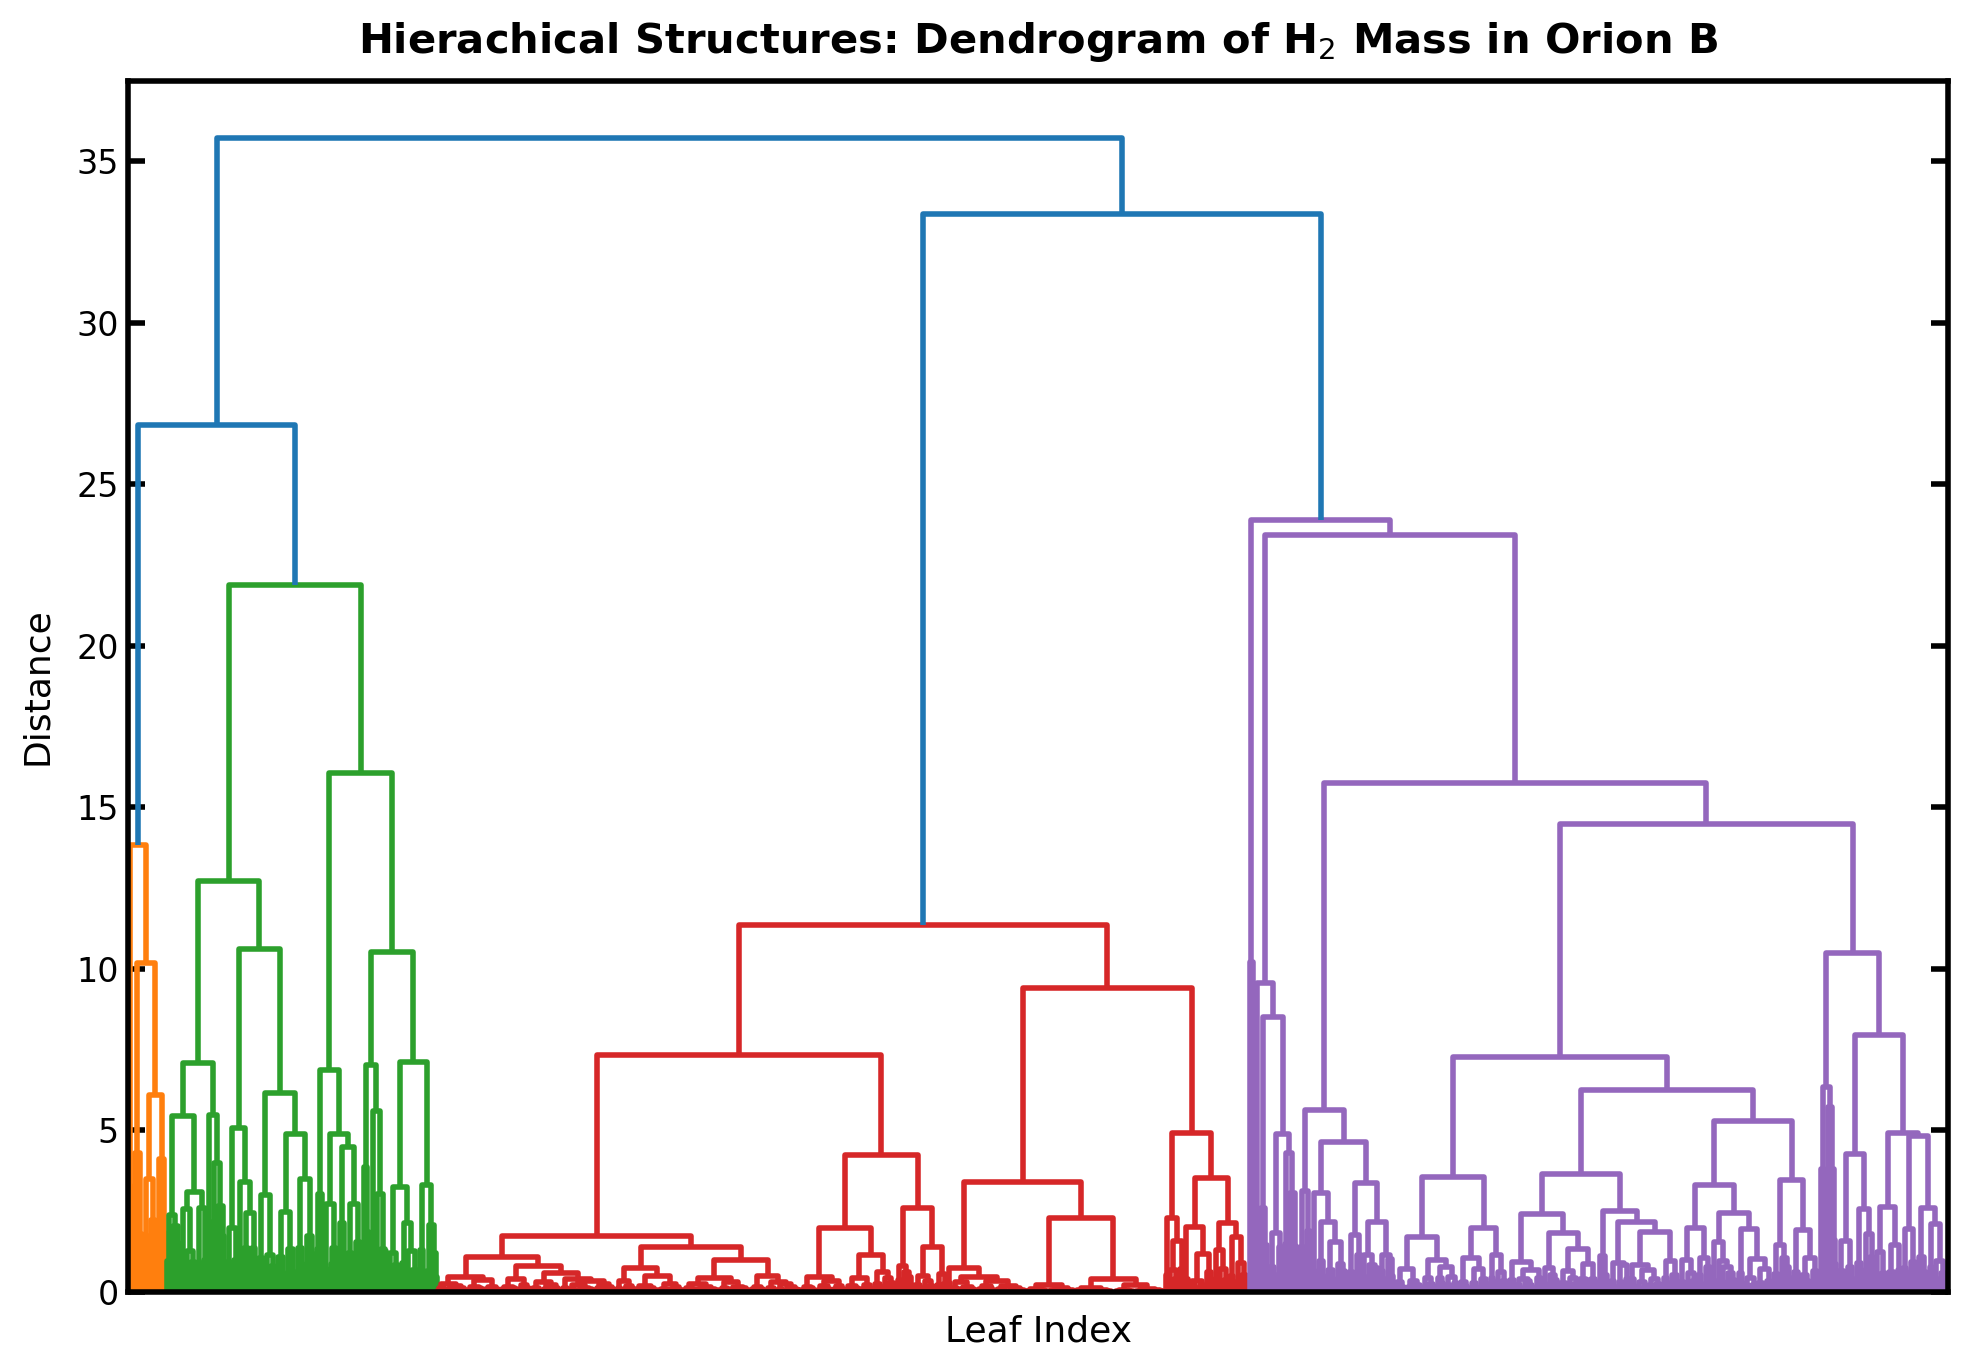
\includegraphics[width=0.5\textwidth]{figures/dendogram_B.png}
    \caption{Dendrogram of the Orion~B mass distribution, showing the hierarchical merging of structures as the column--density threshold is lowered.}
    \label{fig:dendrogram_B}
\end{figure}

We then applied the same calculation of the local fractal dimension to each of these connected structures. For numerical stability, we limited the analysis to the largest regions at each threshold, selecting them according to minimum perimeter and area criteria. The resulting measurements are shown in Figures~\ref{fig:local_A_single_structures} and~\ref{fig:local_B_single_structures}. Overall, these individual--structure analyses reproduce similar trends to those found in the undifferentiated calculation (Figure~\ref{fig:local_Orion_A_B}), although with shallower variations due to the restricted sample.

% To-Do:
% add uncertainties
% make more similar to local Orion A and B
\begin{figure}[t]
    \centering
    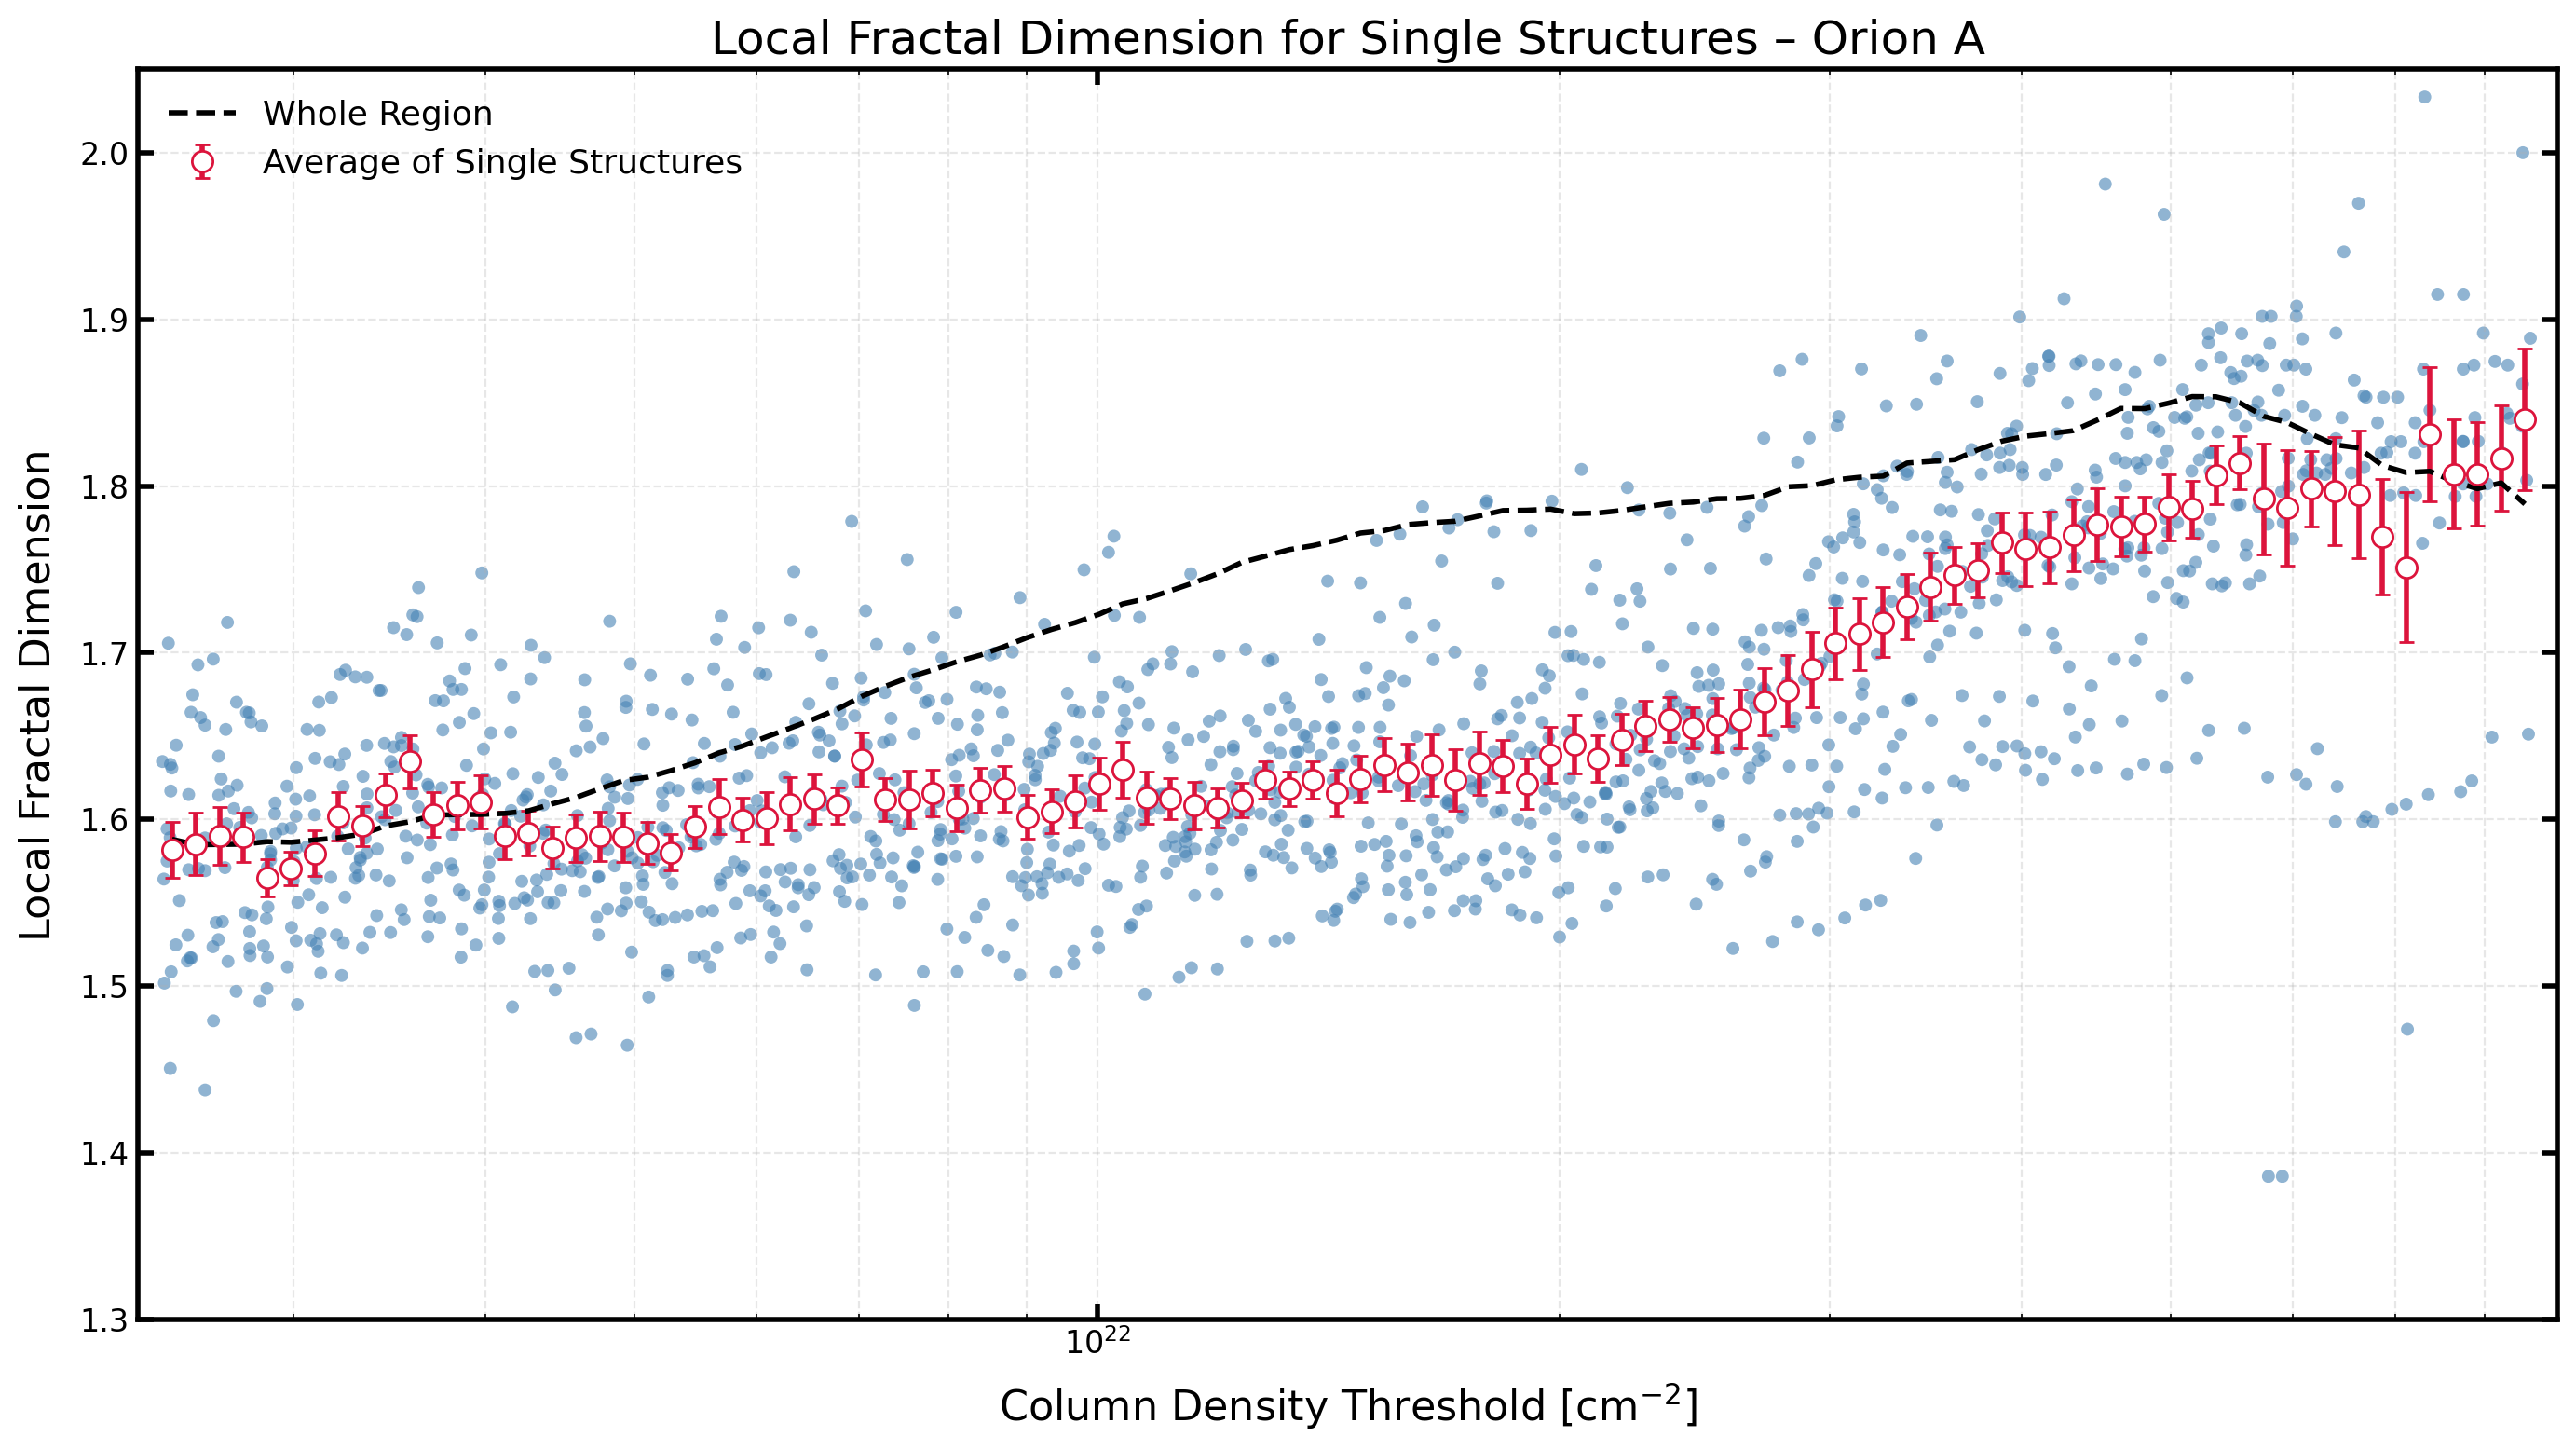
\includegraphics[width=0.5\textwidth]{figures/local_Orion_A_single_structures.png}
    \caption{Local fractal dimension for single structures at each column density threshold for Orion A. Overlaid are both the average of the single regions for each column density threshold as well as the values for the undifferncited calculation. Uncertainties are included.}
    \label{fig:local_A_single_structures}
\end{figure}

\begin{figure}[t]
    \centering
    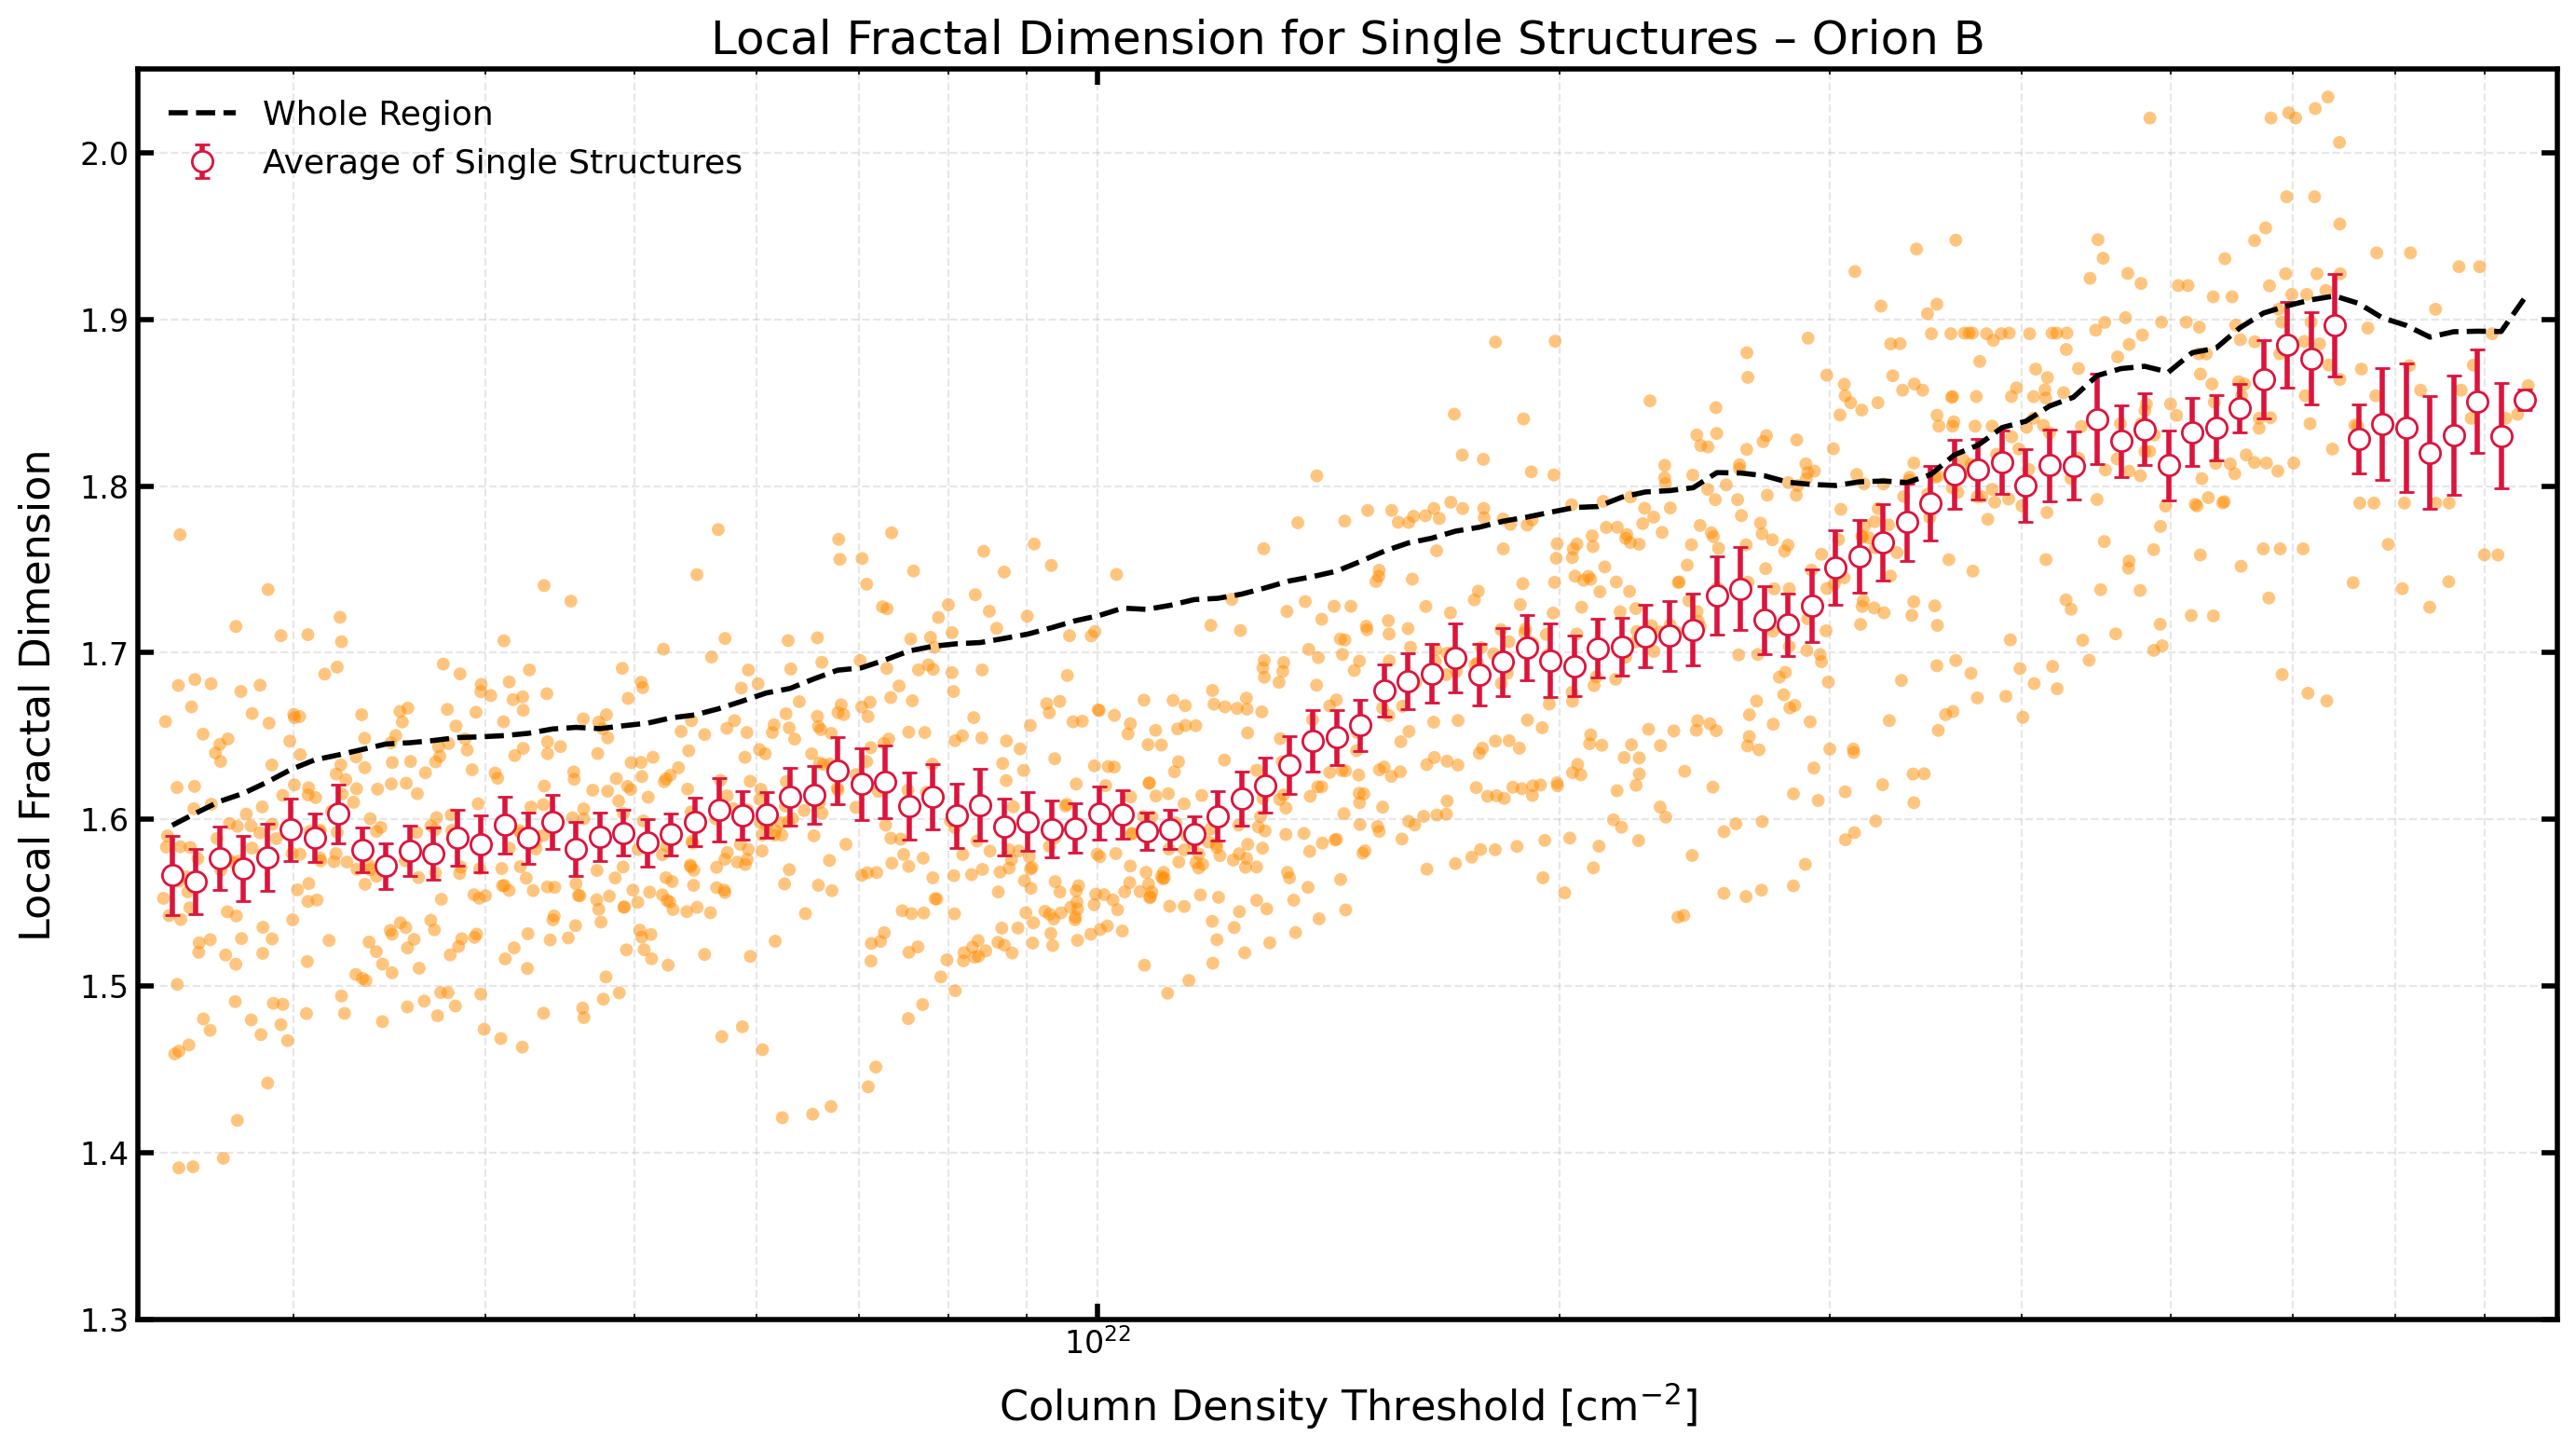
\includegraphics[width=0.5\textwidth]{figures/local_Orion_B_single_structures.png}
    \caption{Local fractal dimension for single structures at each column density threshold for Orion B. Overlaid are both the average of the single regions for each column density threshold as well as the values for the undifferncited calculation. Uncertainties are included.}
    \label{fig:local_B_single_structures}
\end{figure}

\subsection{MSD Plane}

To investigate how the fractal properties relate to the physical characteristics of the cloud, we computed the mass, size, and local fractal dimension for each connected structure identified at every column--density threshold in the dendrogram hierarchy.  
These quantities were then plotted against each other, with the local fractal dimension encoded as color.  
The resulting Mass--Size--Dimension (MSD) planes are shown in Figure~\ref{fig:MSD_orion_A} for Orion~A, Figure~\ref{fig:MSD_orion_B} for Orion~B, and Figure~\ref{fig:MSD_orion_A_B} for the combined dataset.  
For reference, the expected scaling relations for idealized filamentary structures (\(A = 10\)) and spherical structures (\(A = 3\)) are overplotted.

\begin{figure}[t]
    \centering
    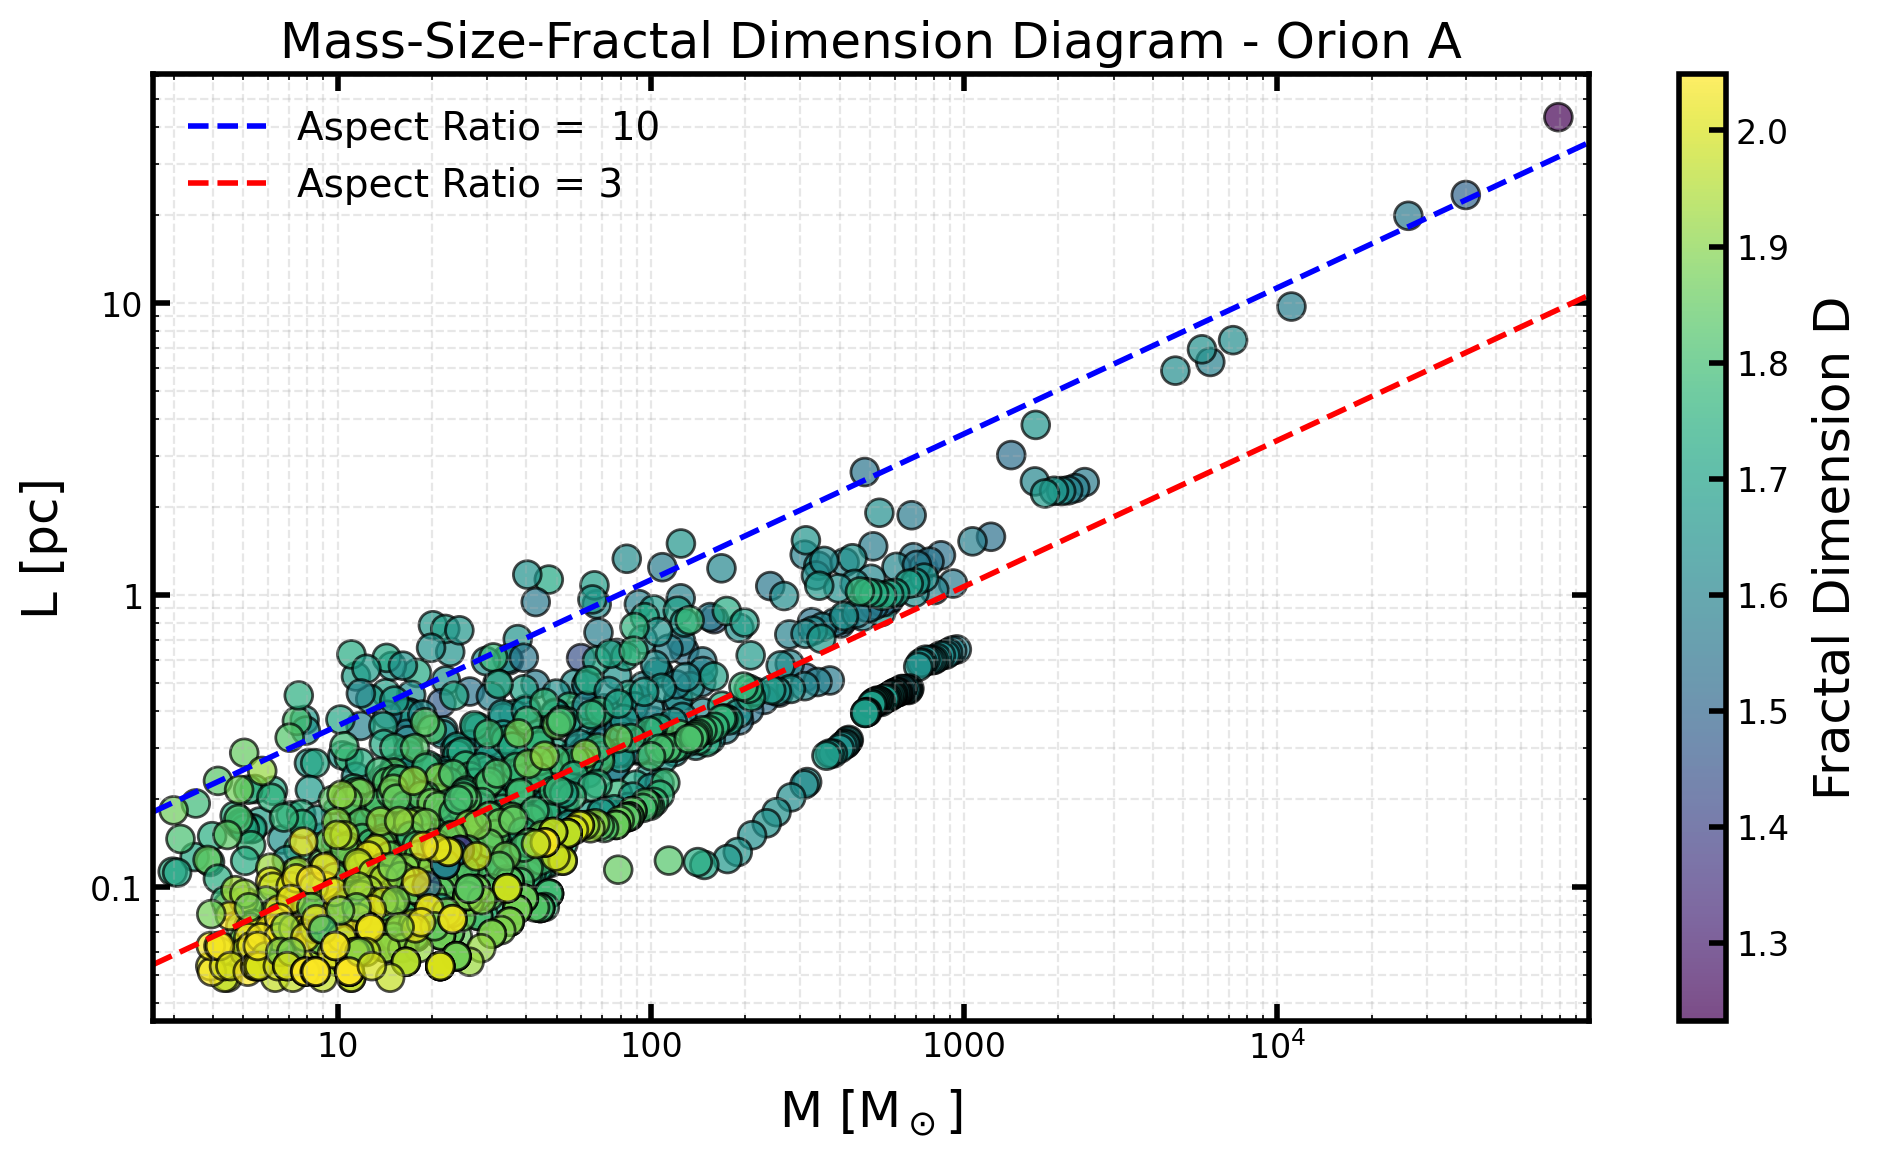
\includegraphics[width=0.6\textwidth]{figures/MSD_Orion_A.png}
    \caption{MSD plane for Orion~A. The color scale indicates the local fractal dimension, and reference scalings for filamentary and spherical geometries are shown as solid lines.}
    \label{fig:MSD_orion_A}
\end{figure}

\begin{figure}[t]
    \centering
    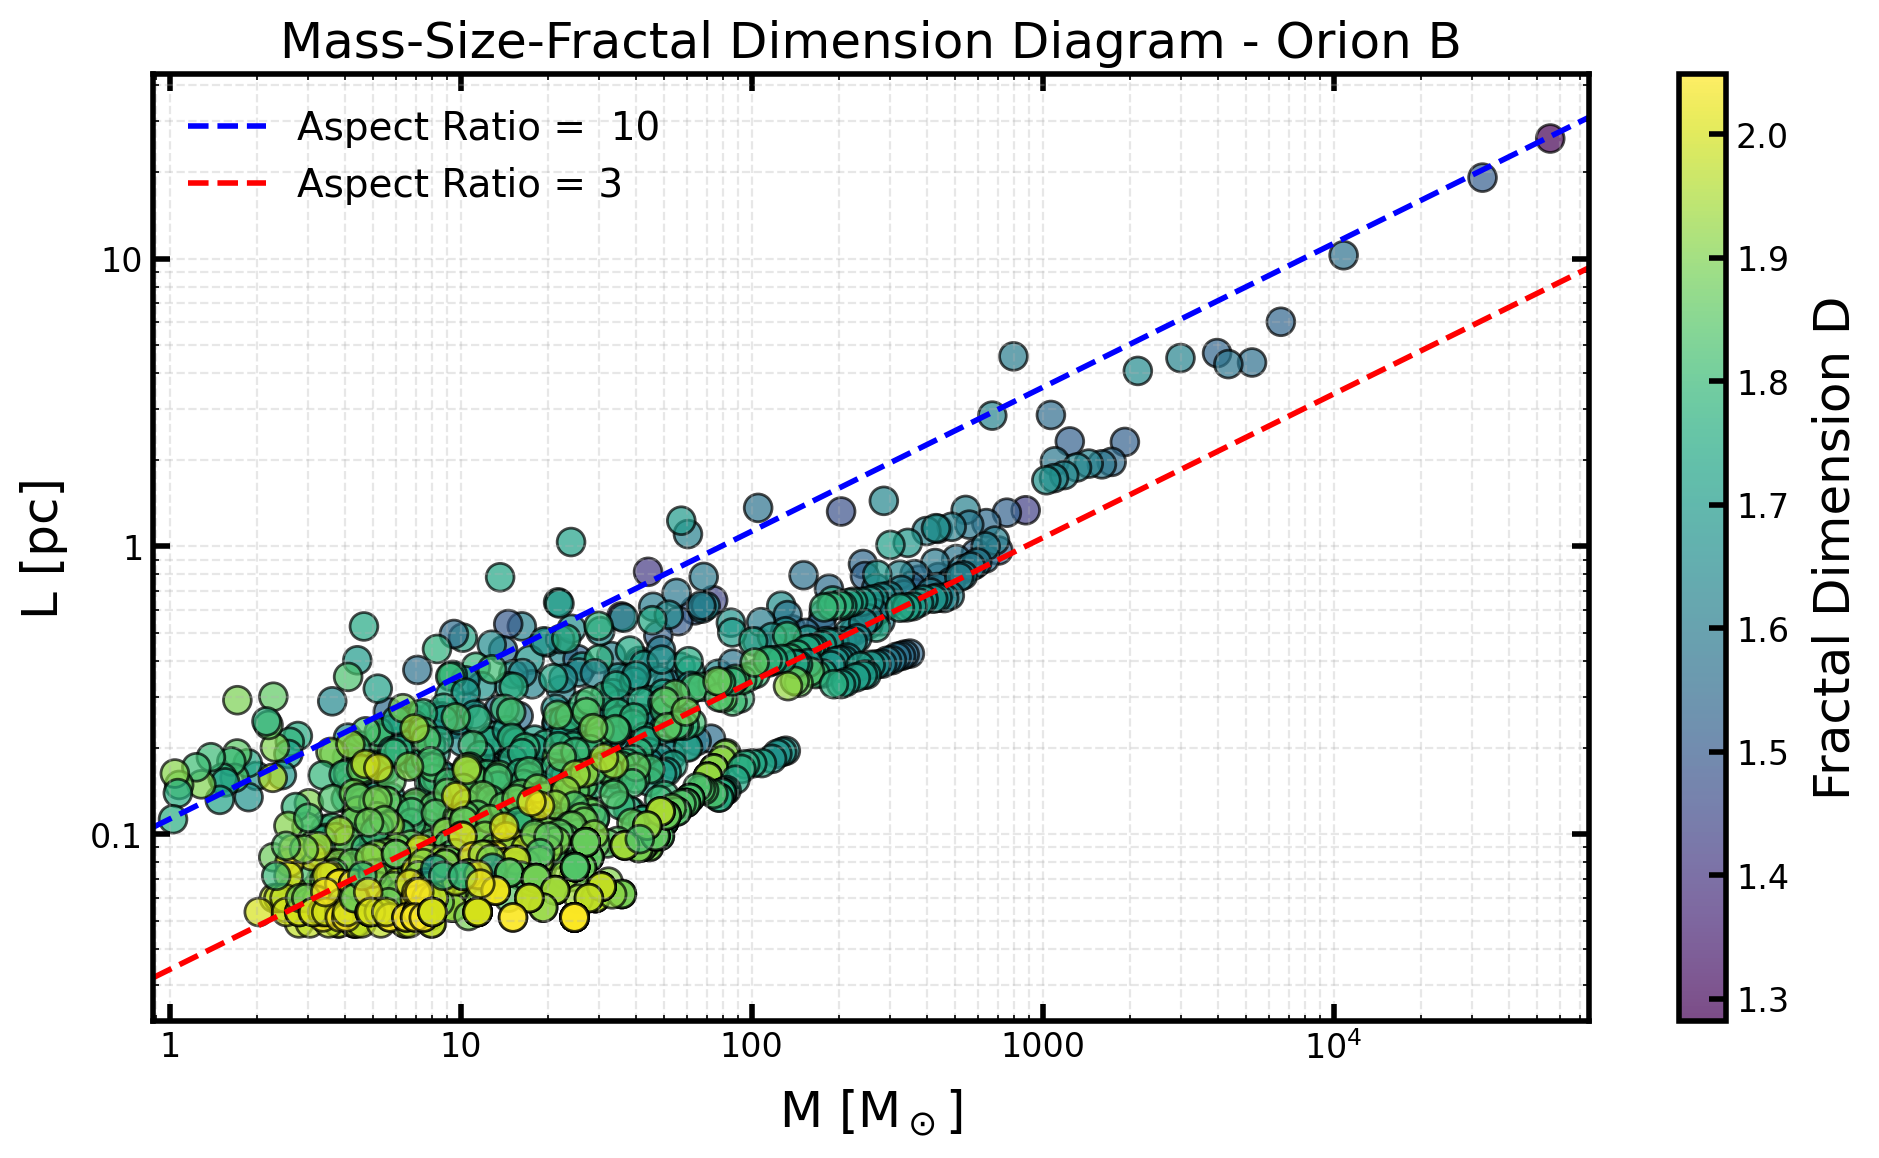
\includegraphics[width=0.6\textwidth]{figures/MSD_Orion_B.png}
    \caption{MSD plane for Orion~B, with the same color coding and reference scalings as in Figure~\ref{fig:MSD_orion_A}.}
    \label{fig:MSD_orion_B}
\end{figure}

\begin{figure}[t]
    \centering
    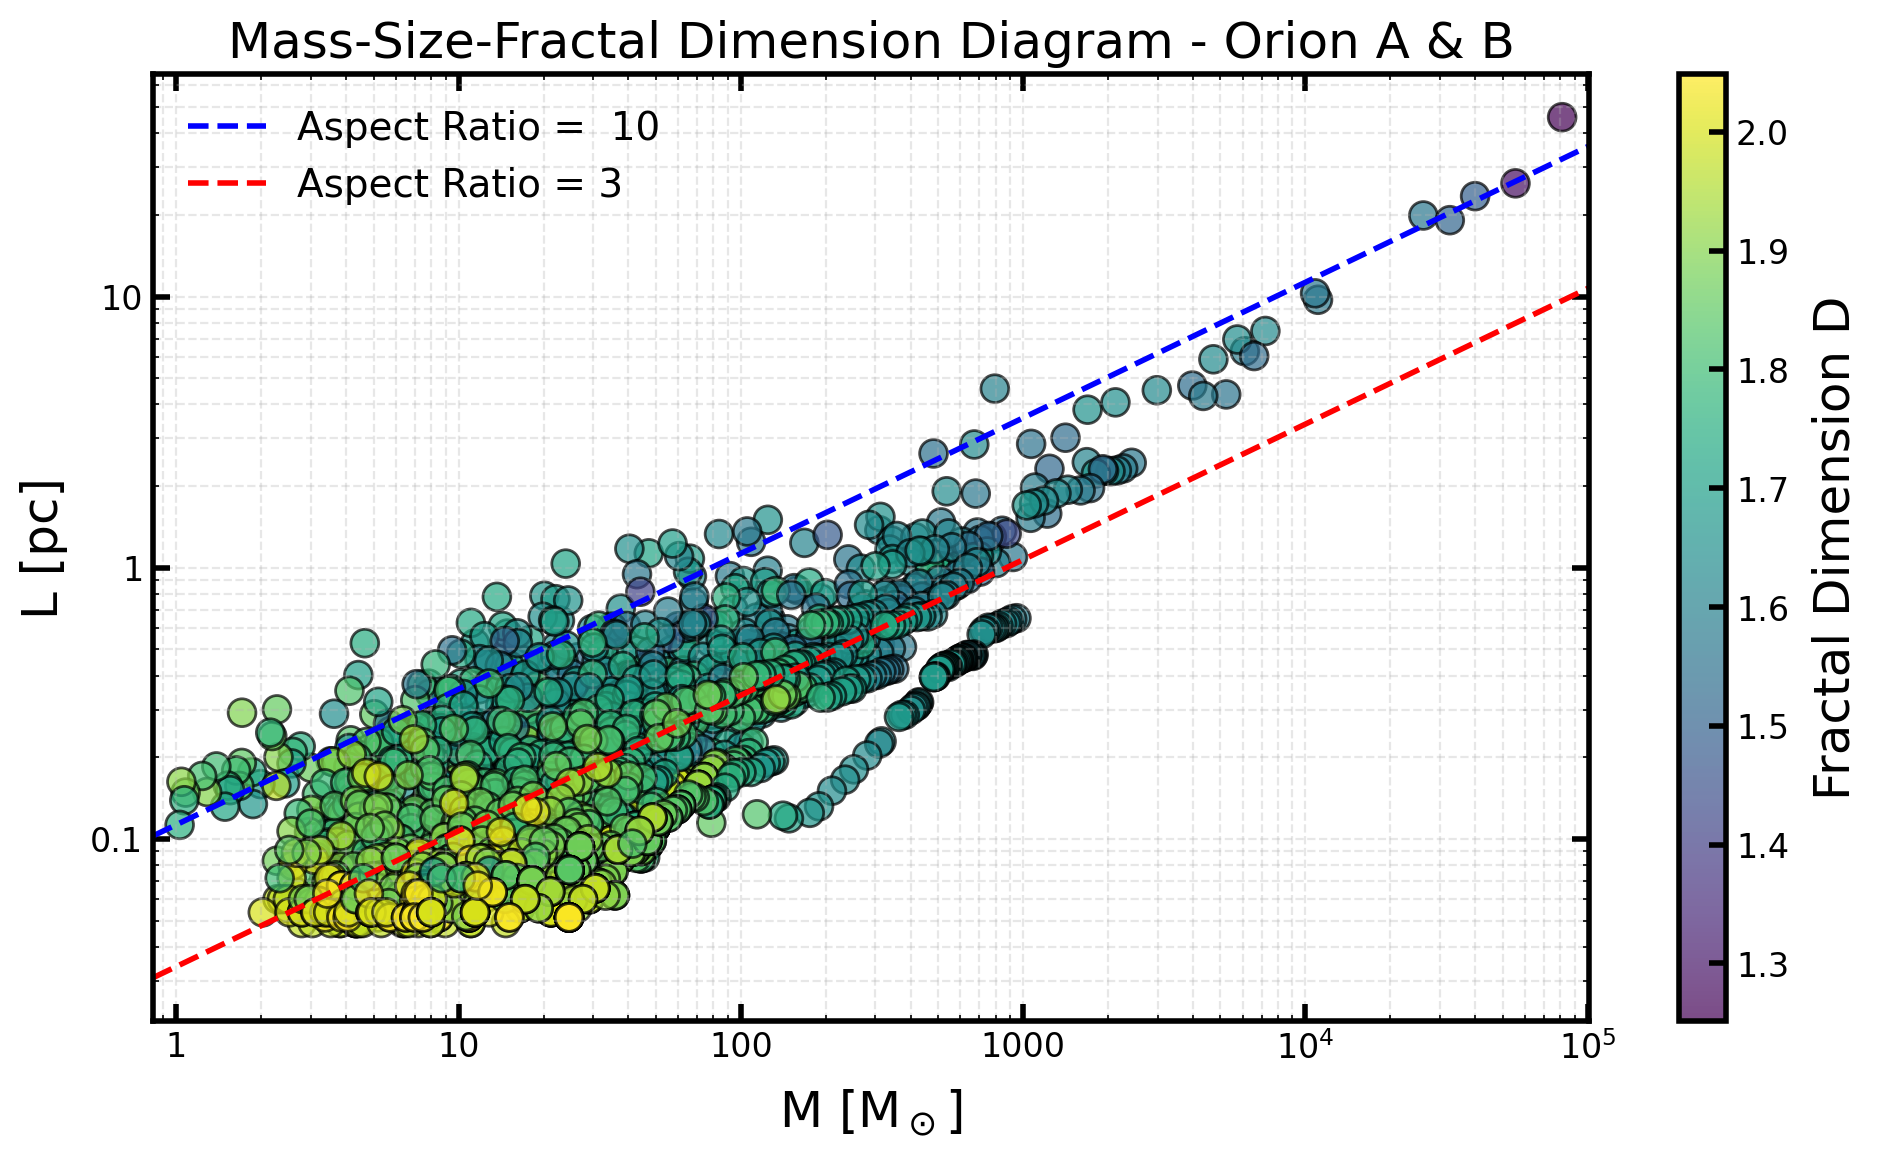
\includegraphics[width=0.6\textwidth]{figures/MSD_Orion_A_B.png}
    \caption{MSD plane for Orion~A and Orion~B combined. The color bar covers the full range of local fractal dimensions across both clouds.}
    \label{fig:MSD_orion_A_B}
\end{figure}

Using this information, we generated spatial maps of the local fractal dimension by assigning to each pixel the value associated with the structure it belongs to.  
If multiple structures overlap, we averaged their values.  
Because of this averaging, the highest values appear slightly reduced compared to the peak values in the previous plots.  
Nevertheless, the maps in Figures~\ref{fig:local_A_map} and~\ref{fig:local_B_map} reinforce the trends already identified in the MSD analysis.

\begin{figure}[t]
    \centering
    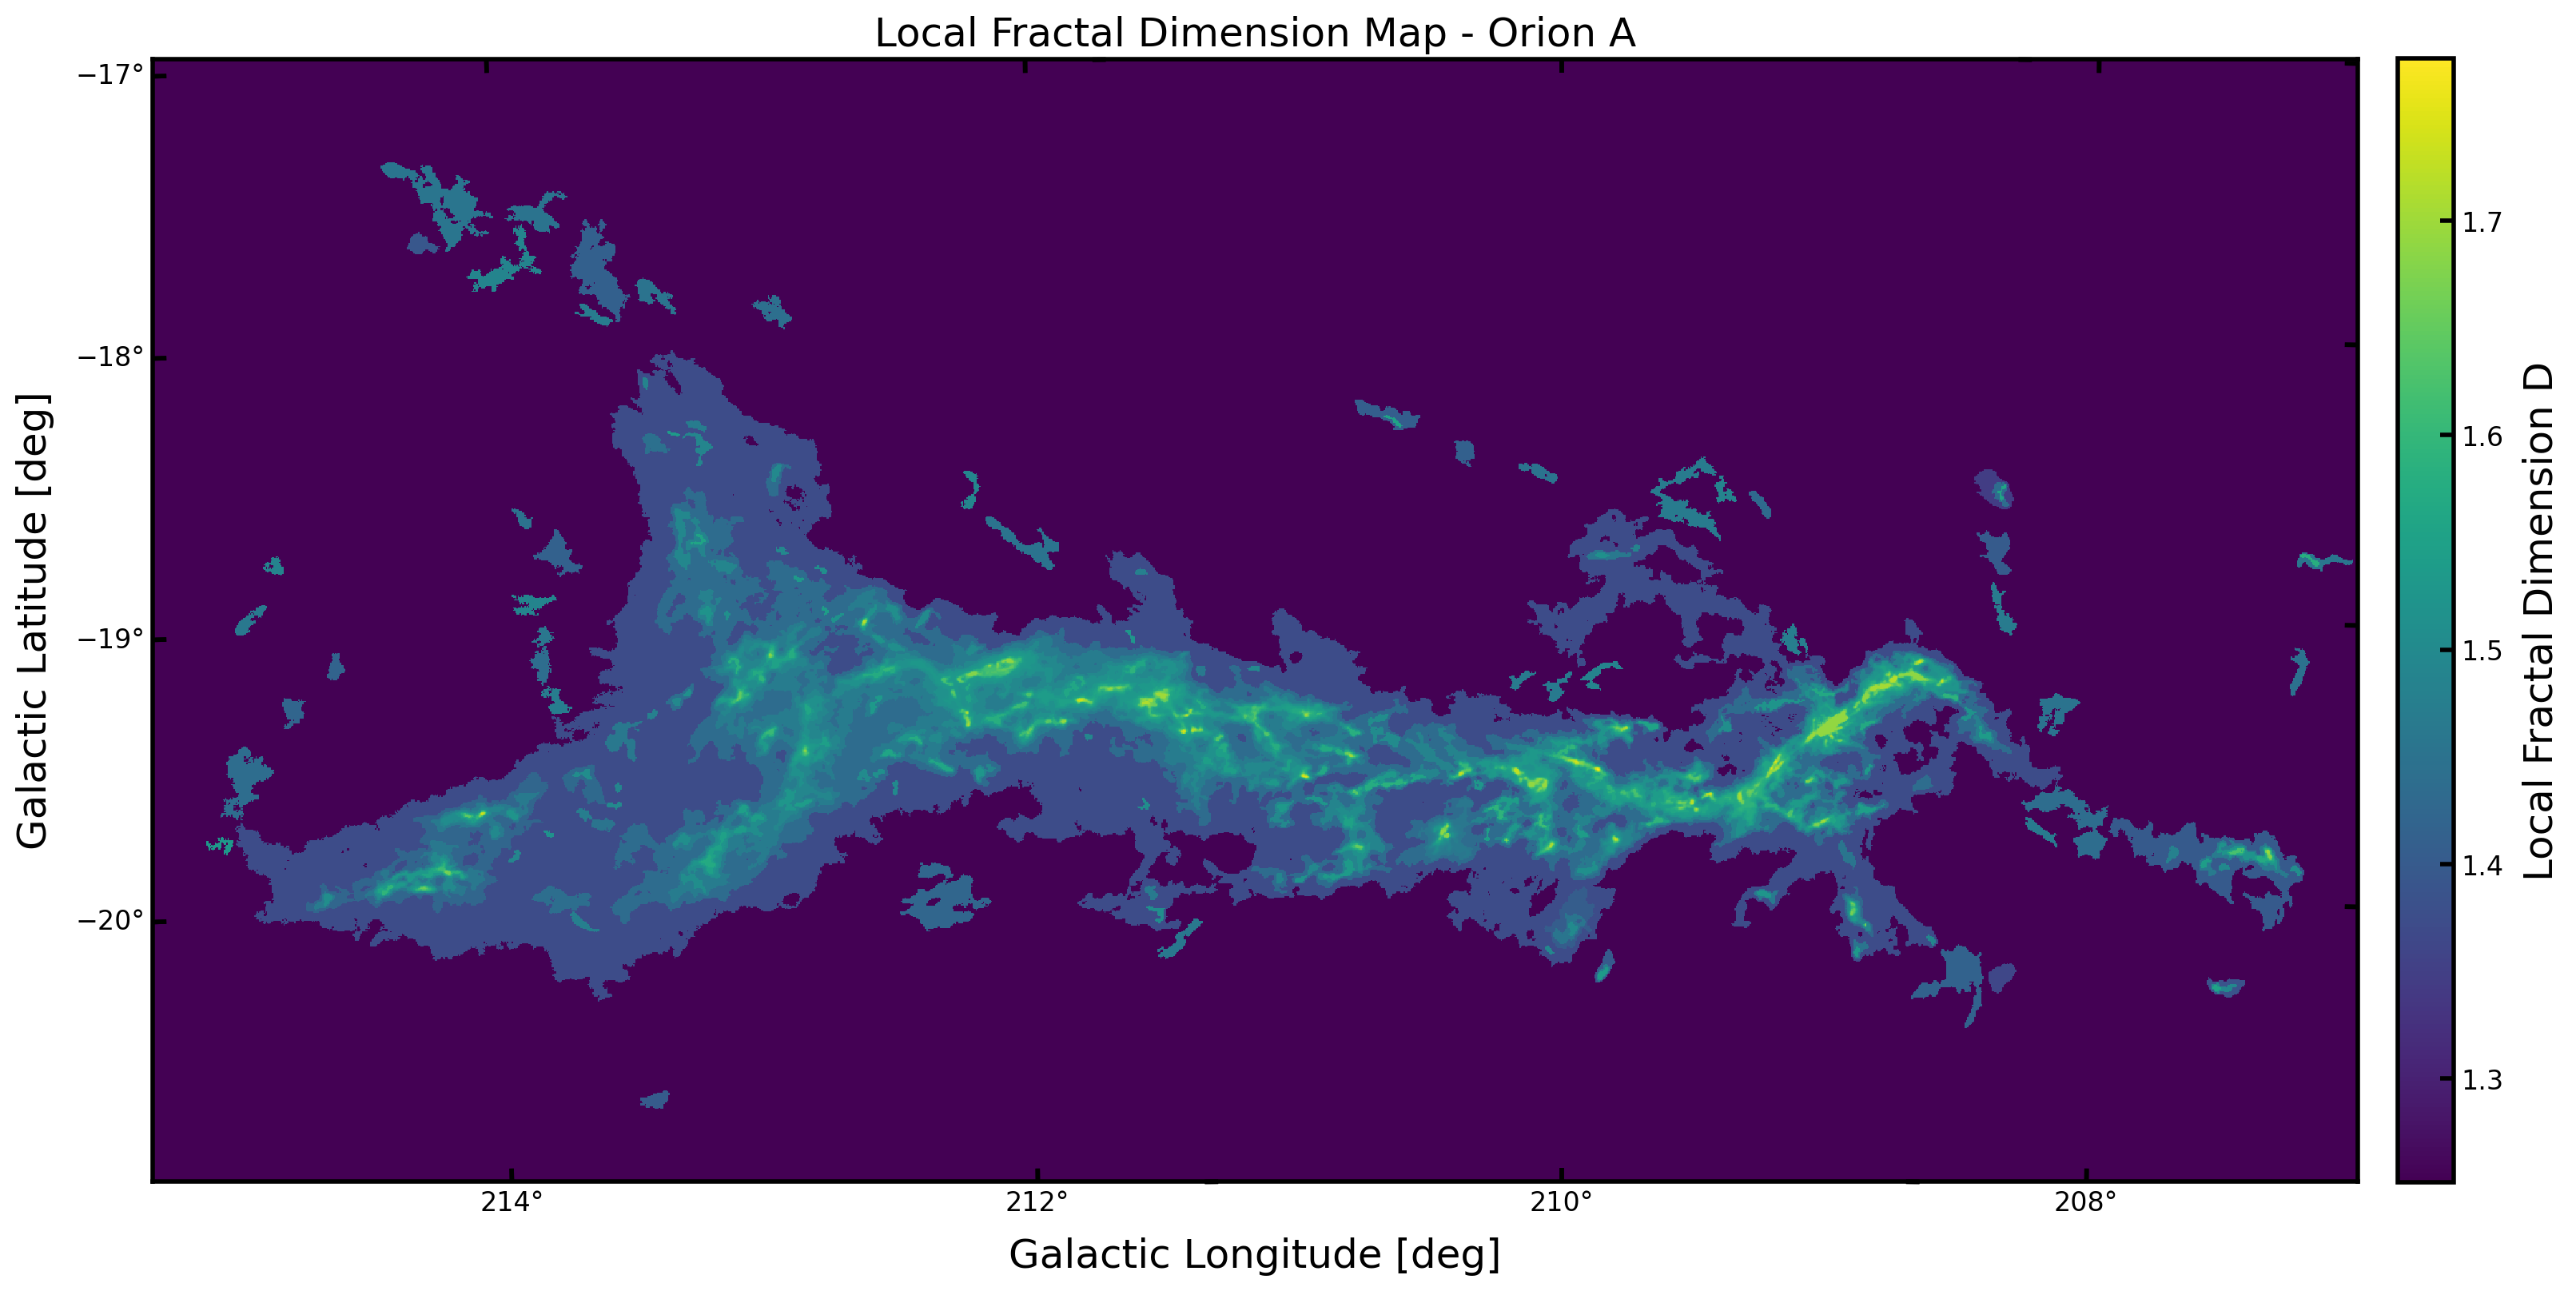
\includegraphics[width=0.6\textwidth]{figures/local_fractal_dimension_map_Orion_A.png}
    \caption{Spatial map of the local fractal dimension for Orion~A. Pixels without assigned structures (NaN) are set to the minimum observed value of the fractal dimension.}
    \label{fig:local_A_map}
\end{figure}

% to-do:
% zoom in (cut the right side)
% remove the straight lines 
\begin{figure}[t]
    \centering
    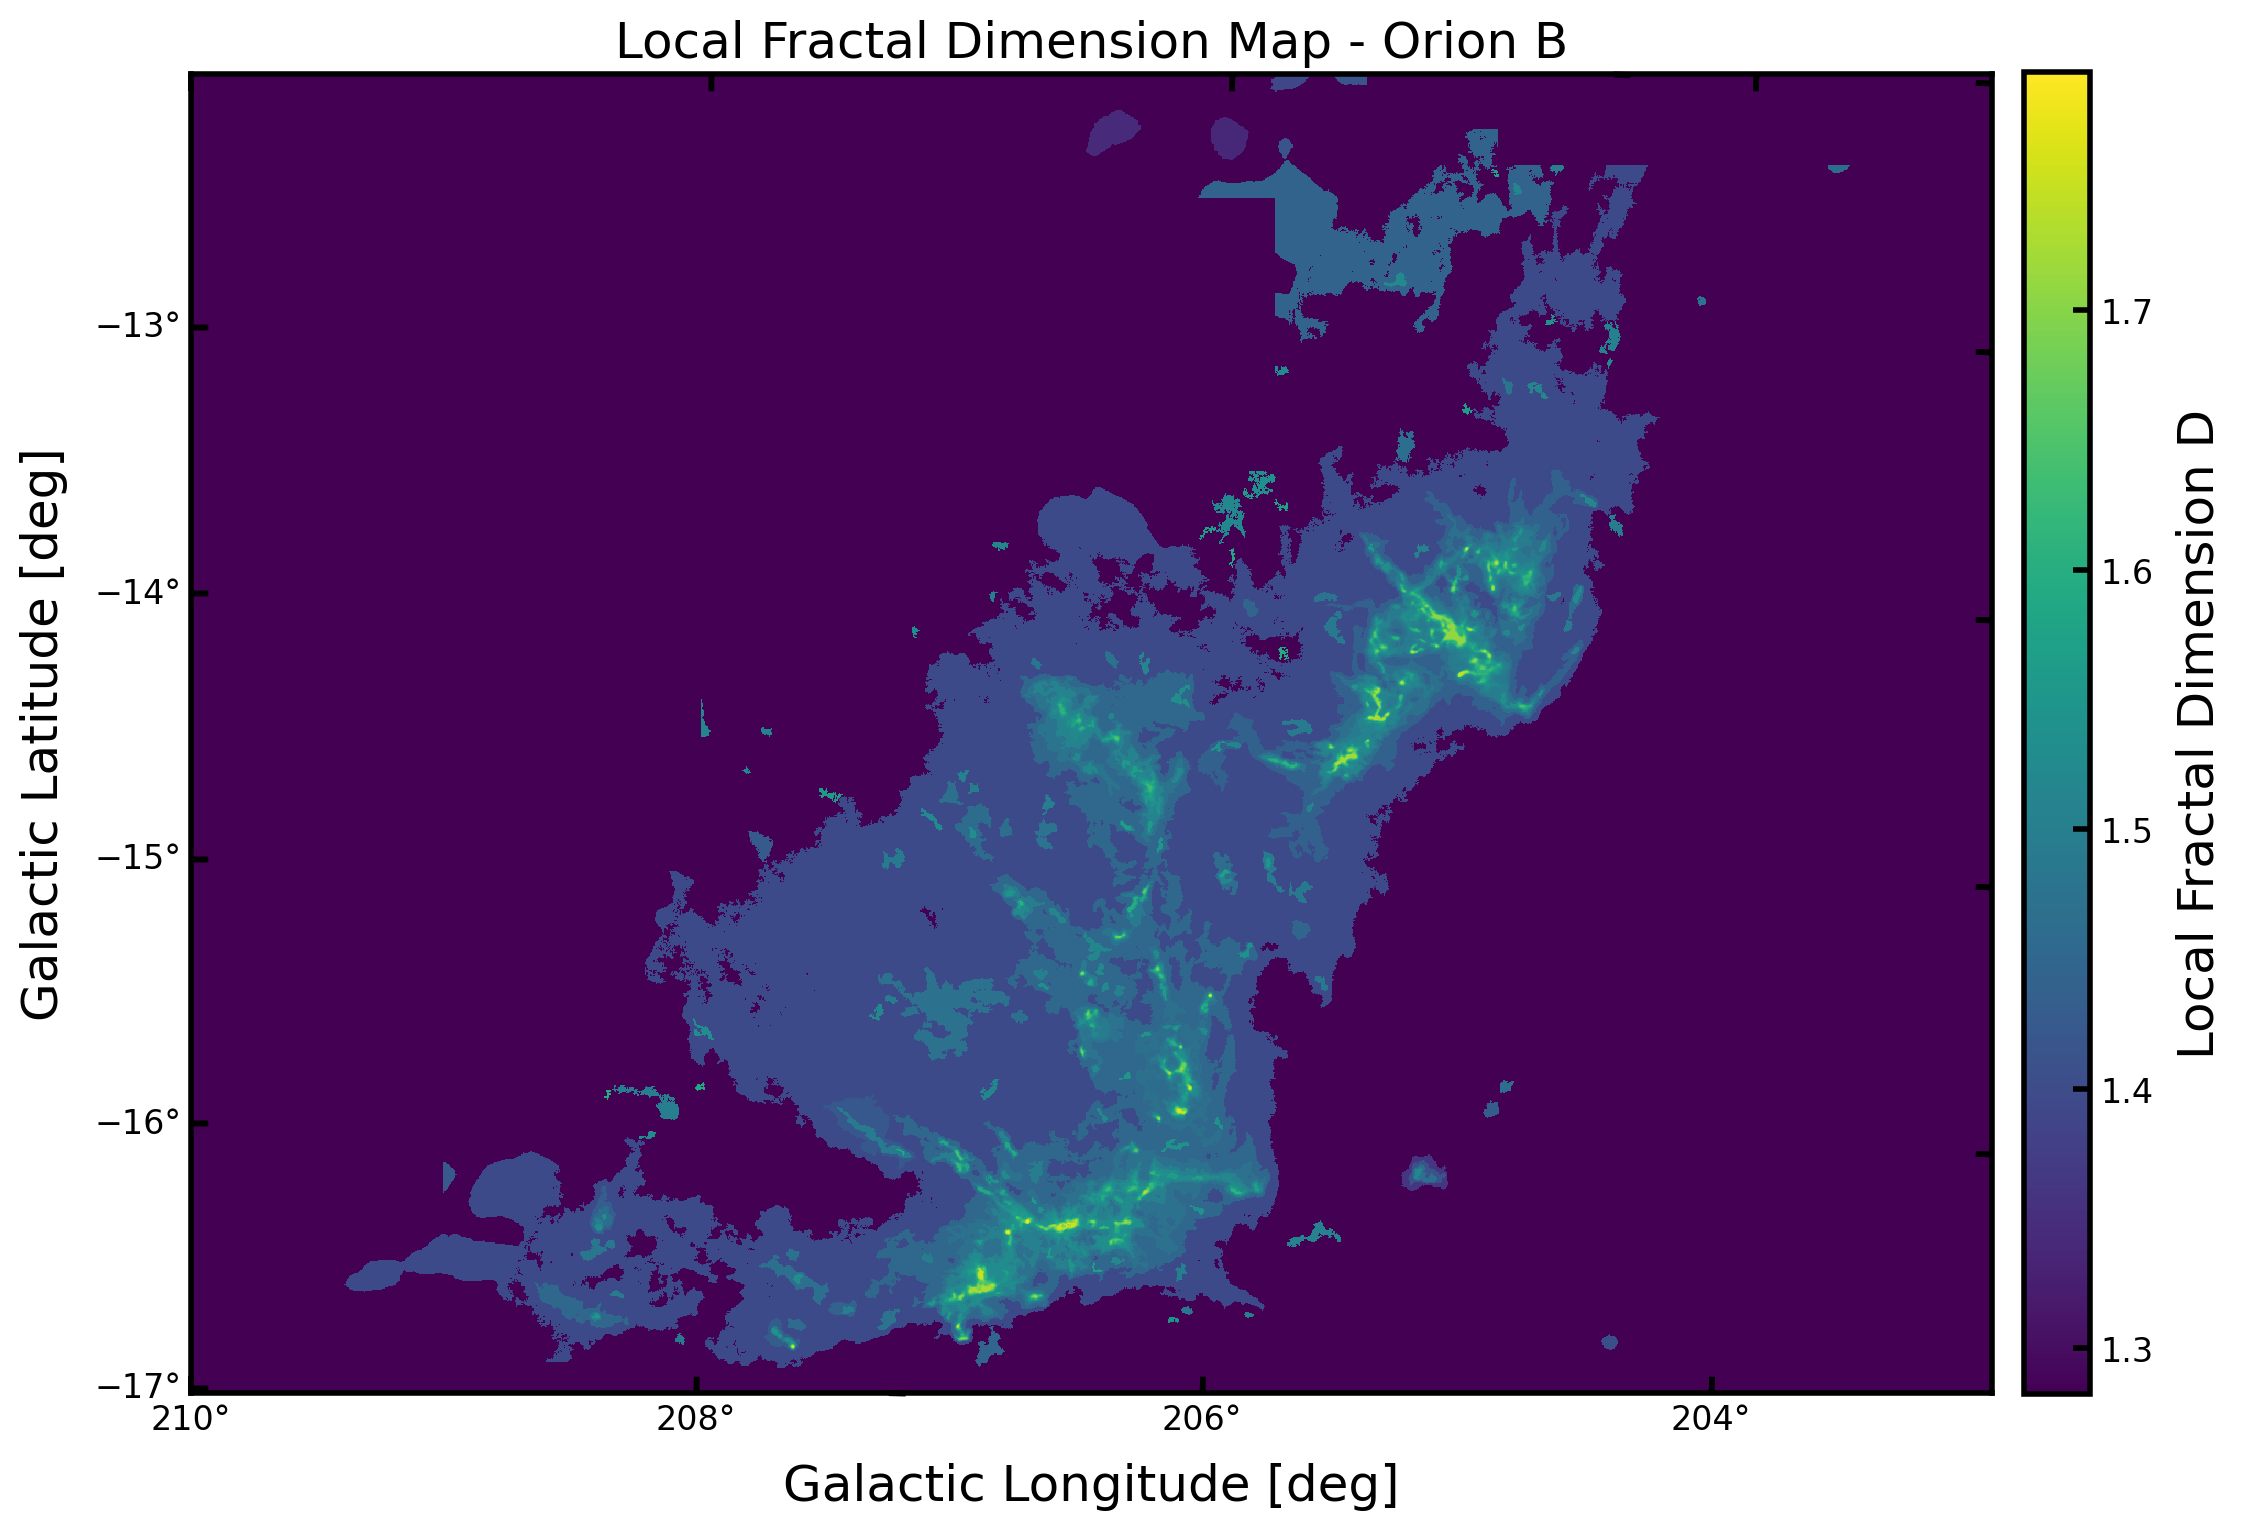
\includegraphics[width=0.6\textwidth]{figures/local_fractal_dimension_map_Orion_B.png}
    \caption{Spatial map of the local fractal dimension for Orion~B. Pixels without assigned structures are set to the minimum observed value.}
    \label{fig:local_B_map}
\end{figure}

An interactive 3D version of the MSD plane is available online at:  
\href{https://simonesped.github.io/MSD_Viz/}{\texttt{MSD-Visualizer}}.

Finally, the hierarchical relationships extracted from the dendrogram allow us to track how individual structures break down into substructures.  
This information is visualized in Figures~\ref{fig:MSD_orion_A_lines} and~\ref{fig:MSD_orion_B_lines}, where lines connect each structure to its parent and child structures in the MSD plane.

% to-do
% likely to redo, very messy
\begin{figure}[t]
    \centering
    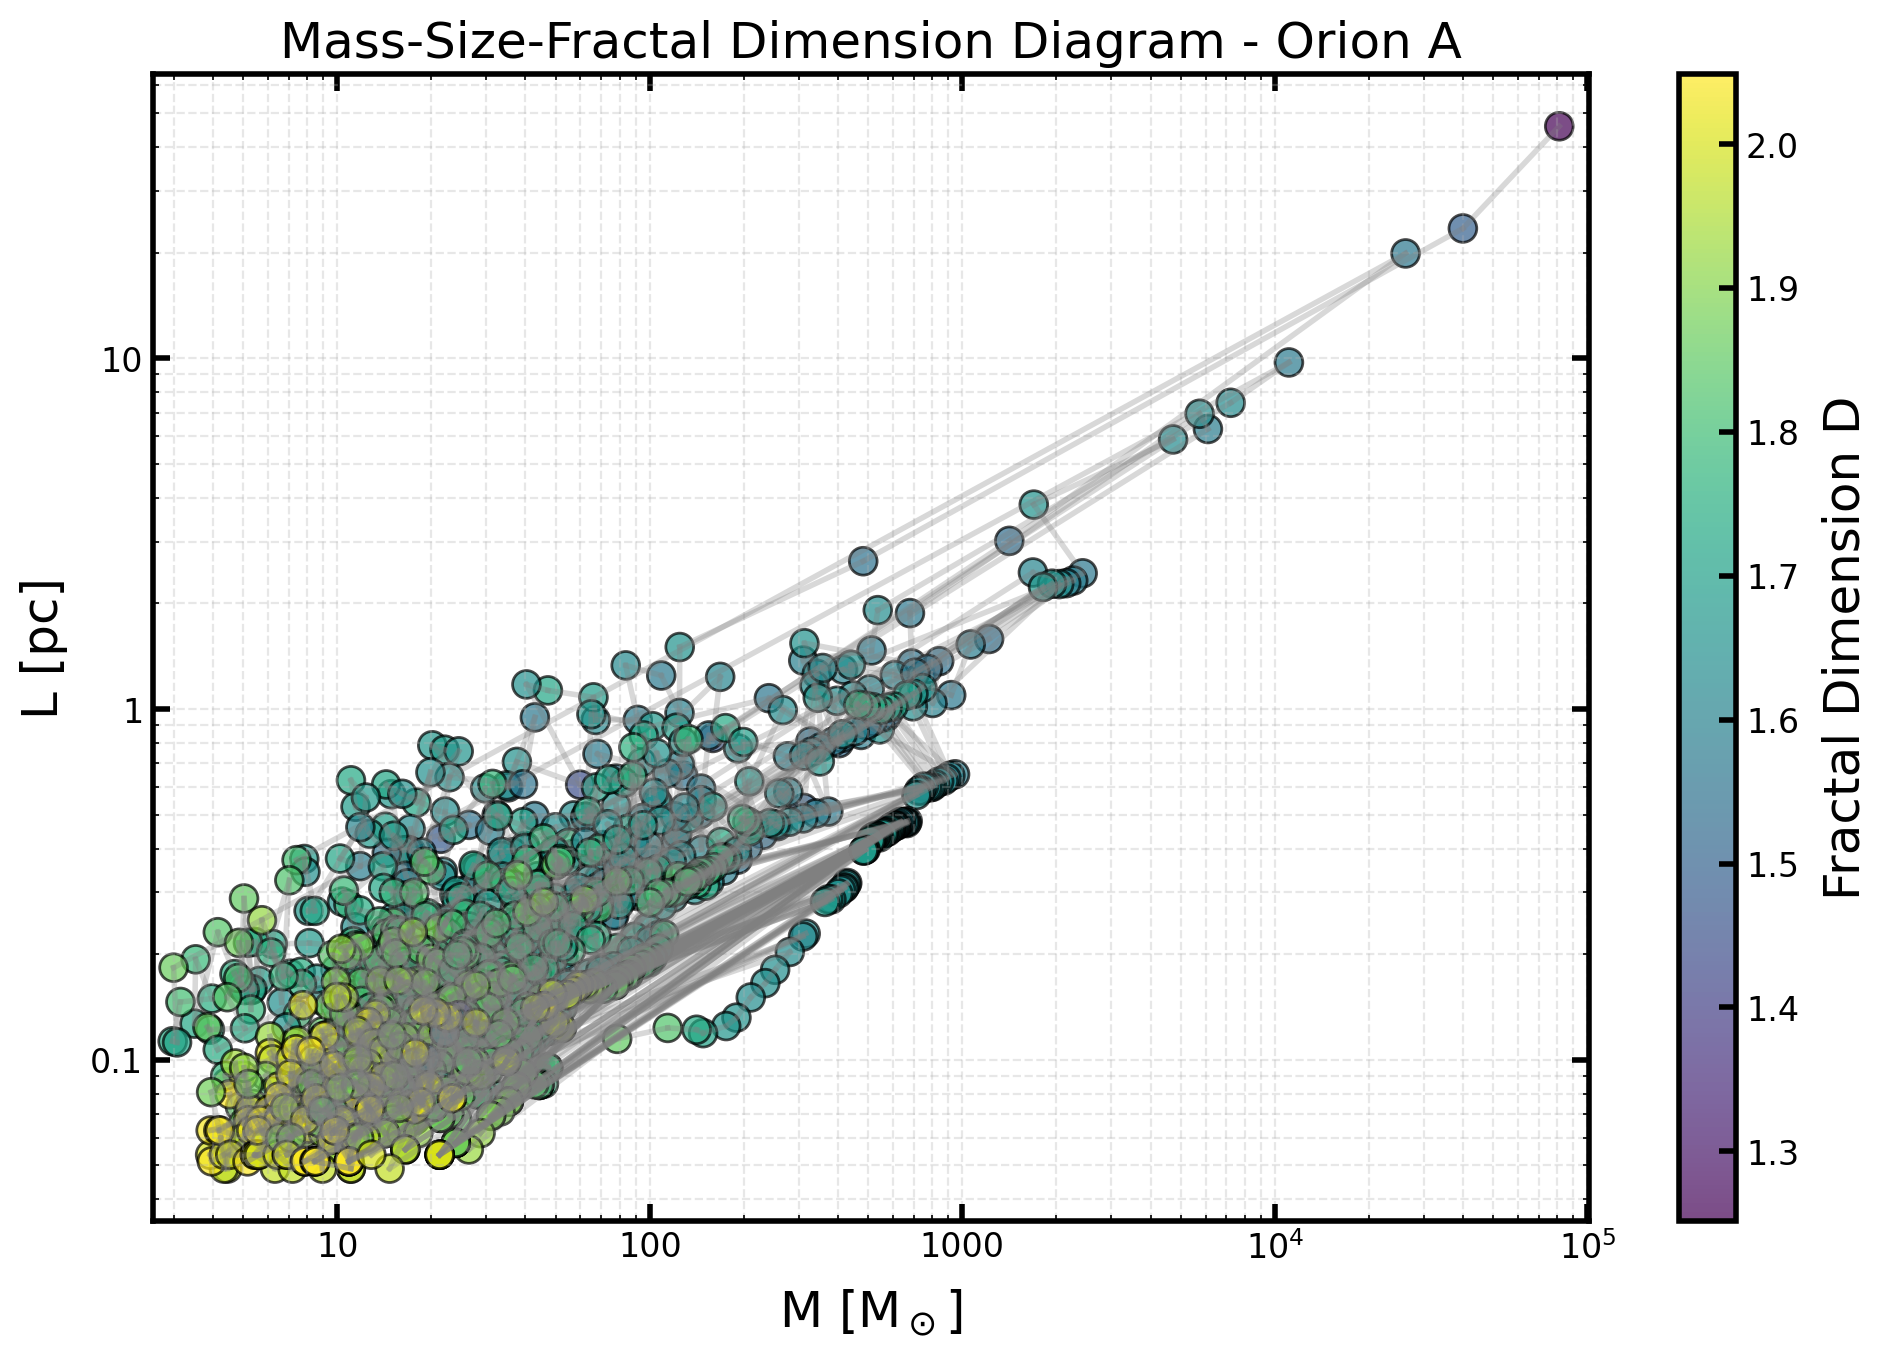
\includegraphics[width=0.5\textwidth]{figures/MSD_Orion_A_with_lines.png}
    \caption{MSD plane for Orion~A with dendrogram connections overplotted. Lines trace parent--child relationships between structures.}
    \label{fig:MSD_orion_A_lines}
\end{figure}

\begin{figure}[t]
    \centering
    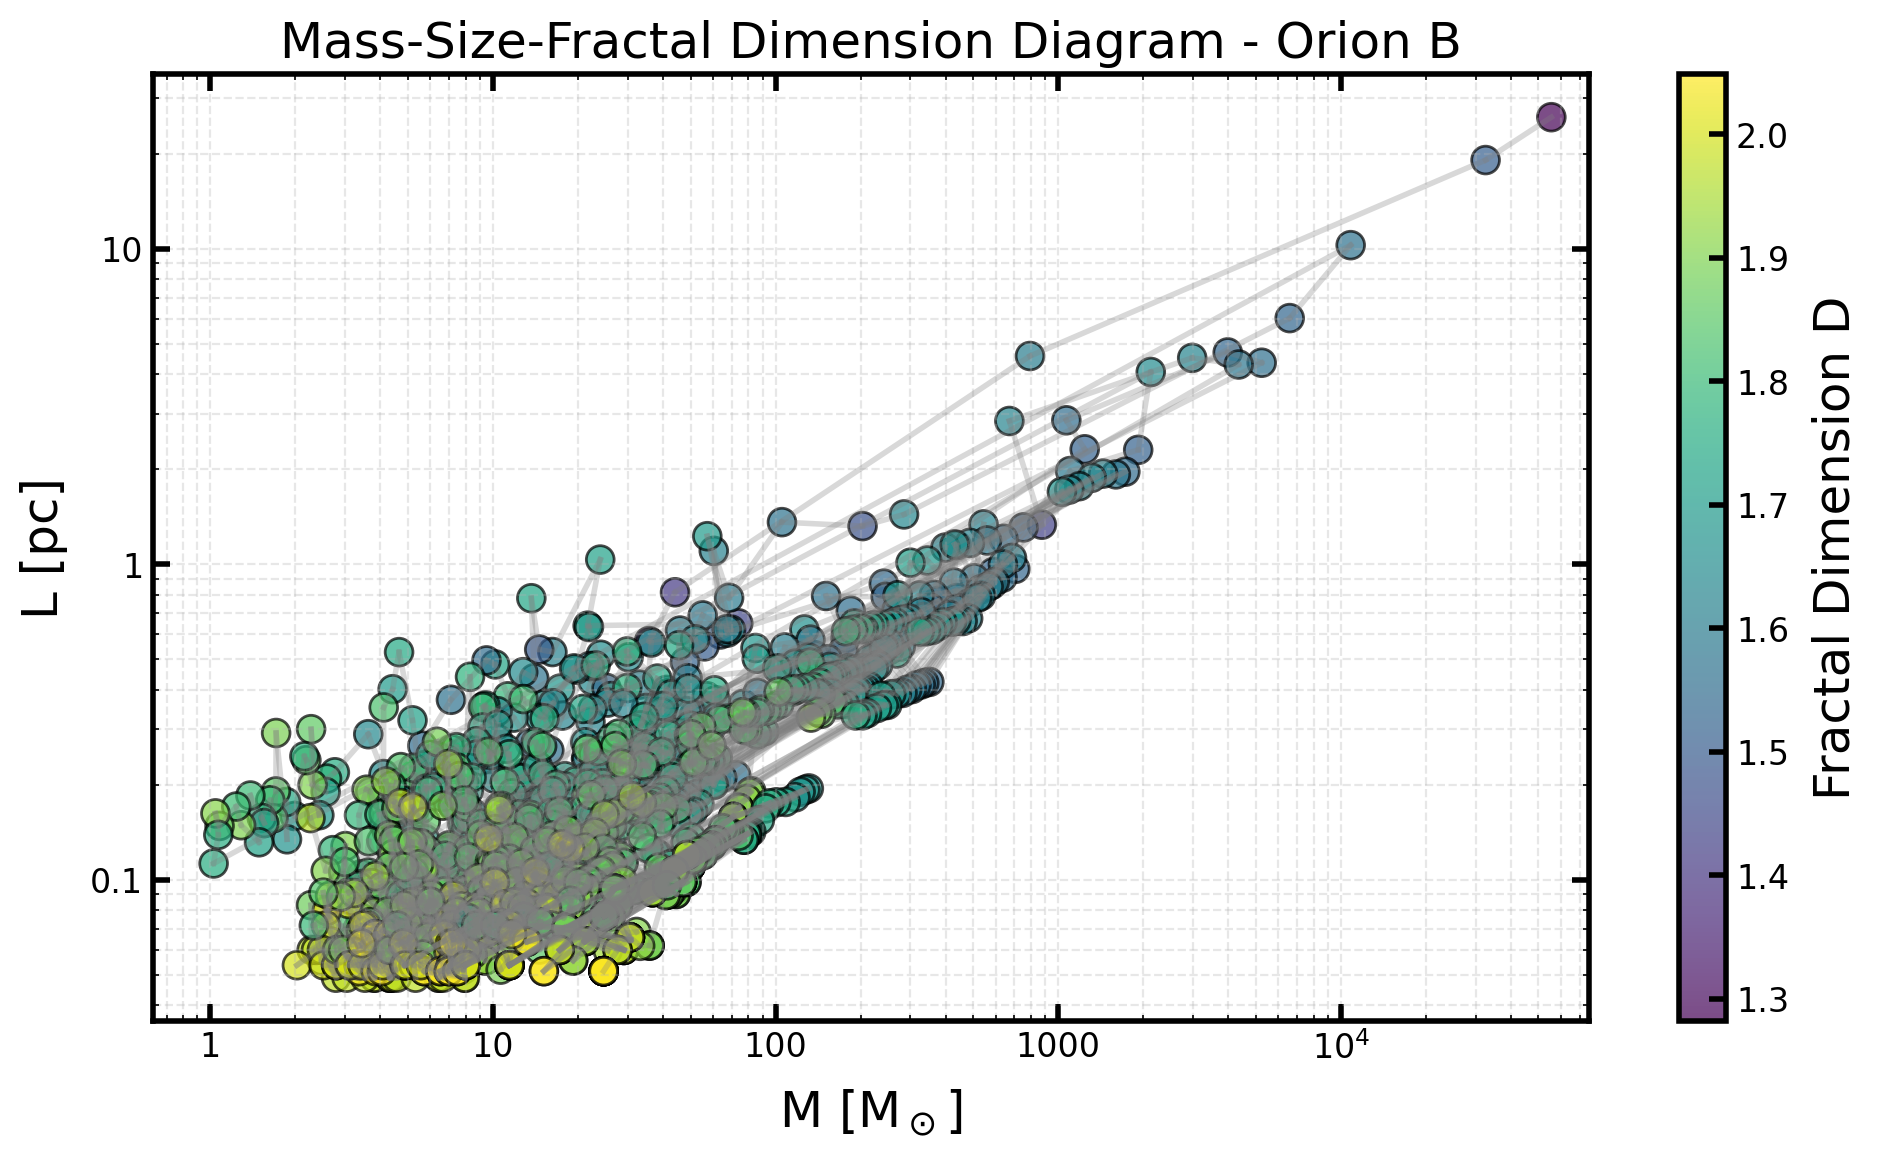
\includegraphics[width=0.5\textwidth]{figures/MSD_Orion_B_with_lines.png}
    \caption{MSD plane for Orion~B with dendrogram connections overplotted.}
    \label{fig:MSD_orion_B_lines}
\end{figure}

% YSOs (which stage of evolution are to be considered?)
\section{Connection to Star Formation}

Regions of higher gas density are expected to be more susceptible to star formation.  
To explore this connection, we compared the spatial distribution of the local fractal dimension with the density of young stellar objects (YSOs).  
The YSO density map was obtained by smoothing the distribution of identified YSOs across the region and is shown in more detail in the APPENDIX (ADD).  
The YSO coverage is limited to the sky area spanned by the available YSO catalogs.

We then performed a pixel-by-pixel comparison between the YSO density map and the local fractal dimension map.  
For Orion~A, the resulting correlation coefficients are:
\[
\text{Pearson: } 0.286, \qquad \text{Spearman: } 0.393.
\]
For Orion~B, we find:
\[
\text{Pearson: } 0.399, \qquad \text{Spearman: } 0.340.
\]

Although the correlations are moderate, these results suggest that regions with higher local fractal dimension---which typically coincide with more complex and denser structures---tend to host a higher surface density of YSOs.  
This supports the idea that the fractal morphology of the cloud is linked to the locations where star formation is more active.

% not a lot of pictures here, rather Appendix
\section{Simulations and Uncertainties}

\subsection{Simulations on Global Properties}

\subsubsection{On the Global Fractal Dimension}

To validate the interpretation of the global fractal dimension framework, we performed a series of controlled tests.  
These tests involved applying the fitting routine to mock structures: some were constructed to exhibit a characteristic scale, while others were explicitly scale-free and therefore self-similar.  
As outlined earlier, the method is expected to return a robust and consistent fit only in the absence of a characteristic scale, which would indicate self-similarity.

We carried out these tests primarily on Gaussian Random Fields (GRFs), exploring both GRFs with power-law spectra (scale-free) and GRFs with peaked spectra (dominated by a characteristic scale).  
The simulations consistently confirmed our expectations, showing that the fitting procedure yields more stable and reliable results in the scale-free case, while deviations appear when a characteristic scale is introduced.

We also tested the impact of resolution effects by smoothing the original data with Gaussian kernels of increasing size.  
Even under extreme smoothing, the resulting global fractal dimension varied by no more than 15--20\,\% relative to the unsmoothed case, indicating that the method is robust within typical observational resolutions. 

\subsection{Simulations on Local Properties}

\subsubsection{On the Euler Characteristic}

To better understand the expected behavior of the Euler characteristic when applied to real data, we performed dedicated simulations.  
As in the previous tests, the main inputs were Gaussian Random Fields (GRFs), chosen for their well-defined statistical properties and the expectation of a symmetric response.  

The simulations confirmed this expectation: the Euler characteristic exhibits a symmetric profile as a function of the threshold, with a clear maximum in connectivity at the central peak and a gradual decrease on either side.  
This behavior closely resembles a Gaussian bell curve, providing a useful reference pattern for interpreting the results from the actual cloud data.

\subsubsection{On the Local Fractal Dimension}
Validity Stuff + Interpretation
Resolution Effects

\subsection{Error estimates}

The uncertainties on the perimeter and area measurements, estimated using the simulation procedures described above, are on average approximately 1.60\% for each quantity. These uncertainties arise primarily from pixelation effects and resolution limitations in the column density maps.  

An example of the resulting error distributions from a representative simulation run is shown in Figure~\ref{fig:uncertainties}. The narrow spread around the mean confirms that the estimates are robust and systematic errors remain small compared to the dynamic range of the measurements.

\begin{figure}[t]
    \centering
    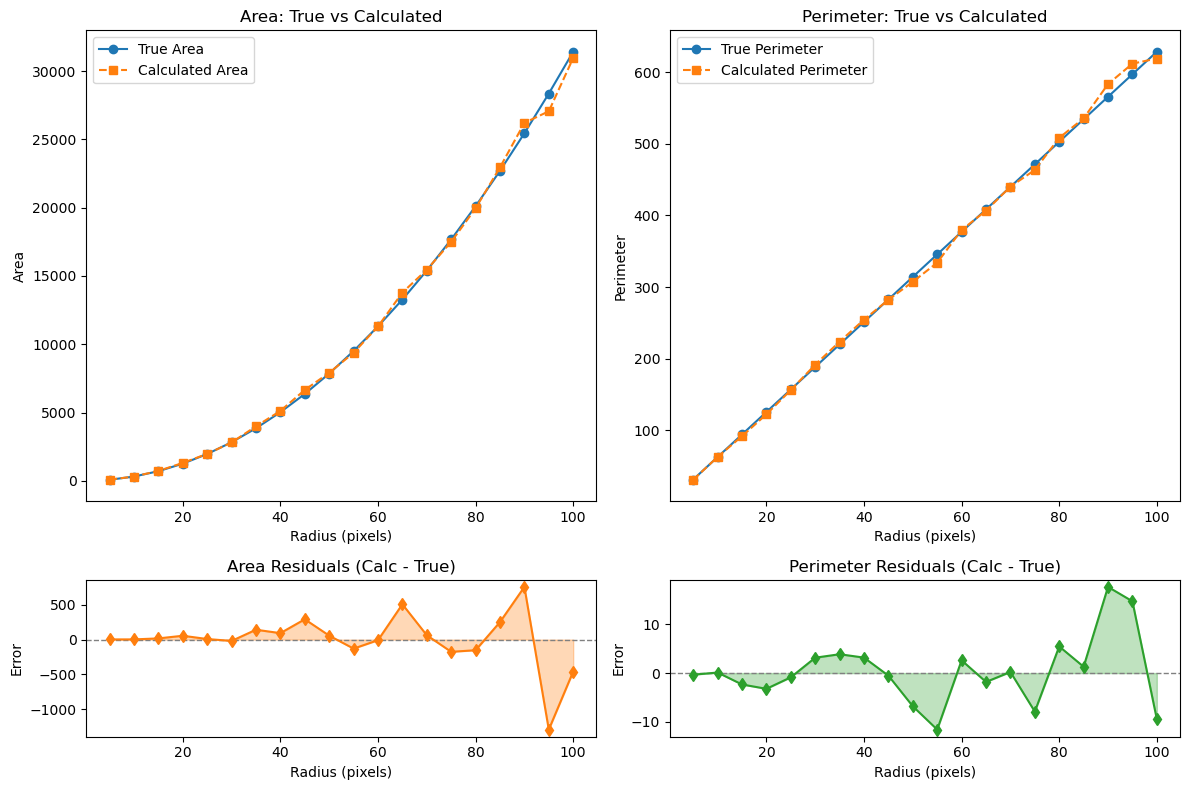
\includegraphics[width=0.75\textwidth]{figures/perimeter_area_uncertainties.png}
    \caption{Example of the uncertainty distributions in the measurements of perimeter and area from simulated structures (arbitrary units).}
    \label{fig:uncertainties}
\end{figure}

\subsection{Comparison with alternative methods}

A clear anti-correlation is observed when comparing results with the box-counting method, both for the global and local estimates of the fractal dimension. This highlights an interesting scaling property that should be taken into account when comparing studies that employ different techniques for quantifying fractal characteristics.
